
% Inherit from the specified cell style.

% Default to the notebook output style

    


% Inherit from the specified cell style.




    
\documentclass[letter,12pt]{article}

    
    
\usepackage[T1]{fontenc}
% Nicer default font (+ math font) than Computer Modern for most use cases
\usepackage{mathpazo}

% Basic figure setup, for now with no caption control since it's done
% automatically by Pandoc (which extracts ![](path) syntax from Markdown).
\usepackage{graphicx}
% Ensure that by default, figures have no caption (until we provide a
% proper Figure object with a Caption API and a way to capture that
% in the conversion process - todo).
% \usepackage{caption}
% \DeclareCaptionLabelFormat{nolabel}{}
% \captionsetup{labelformat=nolabel}

\usepackage{adjustbox} % Used to constrain images to a maximum size 
\usepackage{xcolor} % Allow colors to be defined
\usepackage{enumerate} % Needed for markdown enumerations to work
\usepackage{geometry} % Used to adjust the document margins
\usepackage{amsmath} % Equations
\usepackage{amssymb} % Equations
\usepackage{textcomp} % defines textquotesingle
% Hack from http://tex.stackexchange.com/a/47451/13684:
\AtBeginDocument{%
    \def\PYZsq{\textquotesingle}% Upright quotes in Pygmentized code
}
\usepackage{upquote} % Upright quotes for verbatim code
\usepackage{eurosym} % defines \euro
\usepackage[mathletters]{ucs} % Extended unicode (utf-8) support
\usepackage[utf8x]{inputenc} % Allow utf-8 characters in the tex document
\usepackage{fancyvrb} % verbatim replacement that allows latex
\usepackage{grffile} % extends the file name processing of package graphics 
                     % to support a larger range 
% The hyperref package gives us a pdf with properly built
% internal navigation ('pdf bookmarks' for the table of contents,
% internal cross-reference links, web links for URLs, etc.)
\usepackage{hyperref}
\usepackage{booktabs}  % table support for pandoc > 1.12.2
\usepackage[inline]{enumitem} % IRkernel/repr support (it uses the enumerate* environment)
\usepackage[normalem]{ulem} % ulem is needed to support strikethroughs (\sout)
                            % normalem makes italics be italics, not underlines

\usepackage{natbib}
\usepackage[scr]{rsfso}
\usepackage{bm}
% \usepackage{eulervm}
\usepackage{lineno}
\let\originalleft\left
\let\originalright\right
\def\left#1{\mathopen{}\originalleft#1}
\def\right#1{\originalright#1\mathclose{}}
% \usepackage{commath}
\usepackage{mathtools}
\usepackage{pdflscape}
\usepackage[doublespacing]{setspace}
\usepackage{authblk}



    
    
    
    % Colors for the hyperref package
    \definecolor{urlcolor}{rgb}{0,.145,.698}
    \definecolor{linkcolor}{rgb}{.71,0.21,0.01}
    \definecolor{citecolor}{rgb}{.12,.54,.11}

    % ANSI colors
    \definecolor{ansi-black}{HTML}{3E424D}
    \definecolor{ansi-black-intense}{HTML}{282C36}
    \definecolor{ansi-red}{HTML}{E75C58}
    \definecolor{ansi-red-intense}{HTML}{B22B31}
    \definecolor{ansi-green}{HTML}{00A250}
    \definecolor{ansi-green-intense}{HTML}{007427}
    \definecolor{ansi-yellow}{HTML}{DDB62B}
    \definecolor{ansi-yellow-intense}{HTML}{B27D12}
    \definecolor{ansi-blue}{HTML}{208FFB}
    \definecolor{ansi-blue-intense}{HTML}{0065CA}
    \definecolor{ansi-magenta}{HTML}{D160C4}
    \definecolor{ansi-magenta-intense}{HTML}{A03196}
    \definecolor{ansi-cyan}{HTML}{60C6C8}
    \definecolor{ansi-cyan-intense}{HTML}{258F8F}
    \definecolor{ansi-white}{HTML}{C5C1B4}
    \definecolor{ansi-white-intense}{HTML}{A1A6B2}

    % commands and environments needed by pandoc snippets
    % extracted from the output of `pandoc -s`
    \providecommand{\tightlist}{%
      \setlength{\itemsep}{0pt}\setlength{\parskip}{0pt}}
    \DefineVerbatimEnvironment{Highlighting}{Verbatim}{commandchars=\\\{\}}
    % Add ',fontsize=\small' for more characters per line
    \newenvironment{Shaded}{}{}
    \newcommand{\KeywordTok}[1]{\textcolor[rgb]{0.00,0.44,0.13}{\textbf{{#1}}}}
    \newcommand{\DataTypeTok}[1]{\textcolor[rgb]{0.56,0.13,0.00}{{#1}}}
    \newcommand{\DecValTok}[1]{\textcolor[rgb]{0.25,0.63,0.44}{{#1}}}
    \newcommand{\BaseNTok}[1]{\textcolor[rgb]{0.25,0.63,0.44}{{#1}}}
    \newcommand{\FloatTok}[1]{\textcolor[rgb]{0.25,0.63,0.44}{{#1}}}
    \newcommand{\CharTok}[1]{\textcolor[rgb]{0.25,0.44,0.63}{{#1}}}
    \newcommand{\StringTok}[1]{\textcolor[rgb]{0.25,0.44,0.63}{{#1}}}
    \newcommand{\CommentTok}[1]{\textcolor[rgb]{0.38,0.63,0.69}{\textit{{#1}}}}
    \newcommand{\OtherTok}[1]{\textcolor[rgb]{0.00,0.44,0.13}{{#1}}}
    \newcommand{\AlertTok}[1]{\textcolor[rgb]{1.00,0.00,0.00}{\textbf{{#1}}}}
    \newcommand{\FunctionTok}[1]{\textcolor[rgb]{0.02,0.16,0.49}{{#1}}}
    \newcommand{\RegionMarkerTok}[1]{{#1}}
    \newcommand{\ErrorTok}[1]{\textcolor[rgb]{1.00,0.00,0.00}{\textbf{{#1}}}}
    \newcommand{\NormalTok}[1]{{#1}}
    
    % Additional commands for more recent versions of Pandoc
    \newcommand{\ConstantTok}[1]{\textcolor[rgb]{0.53,0.00,0.00}{{#1}}}
    \newcommand{\SpecialCharTok}[1]{\textcolor[rgb]{0.25,0.44,0.63}{{#1}}}
    \newcommand{\VerbatimStringTok}[1]{\textcolor[rgb]{0.25,0.44,0.63}{{#1}}}
    \newcommand{\SpecialStringTok}[1]{\textcolor[rgb]{0.73,0.40,0.53}{{#1}}}
    \newcommand{\ImportTok}[1]{{#1}}
    \newcommand{\DocumentationTok}[1]{\textcolor[rgb]{0.73,0.13,0.13}{\textit{{#1}}}}
    \newcommand{\AnnotationTok}[1]{\textcolor[rgb]{0.38,0.63,0.69}{\textbf{\textit{{#1}}}}}
    \newcommand{\CommentVarTok}[1]{\textcolor[rgb]{0.38,0.63,0.69}{\textbf{\textit{{#1}}}}}
    \newcommand{\VariableTok}[1]{\textcolor[rgb]{0.10,0.09,0.49}{{#1}}}
    \newcommand{\ControlFlowTok}[1]{\textcolor[rgb]{0.00,0.44,0.13}{\textbf{{#1}}}}
    \newcommand{\OperatorTok}[1]{\textcolor[rgb]{0.40,0.40,0.40}{{#1}}}
    \newcommand{\BuiltInTok}[1]{{#1}}
    \newcommand{\ExtensionTok}[1]{{#1}}
    \newcommand{\PreprocessorTok}[1]{\textcolor[rgb]{0.74,0.48,0.00}{{#1}}}
    \newcommand{\AttributeTok}[1]{\textcolor[rgb]{0.49,0.56,0.16}{{#1}}}
    \newcommand{\InformationTok}[1]{\textcolor[rgb]{0.38,0.63,0.69}{\textbf{\textit{{#1}}}}}
    \newcommand{\WarningTok}[1]{\textcolor[rgb]{0.38,0.63,0.69}{\textbf{\textit{{#1}}}}}
    
    
    % Define a nice break command that doesn't care if a line doesn't already
    % exist.
    \def\br{\hspace*{\fill} \\* }
    % Math Jax compatability definitions
    \def\gt{>}
    \def\lt{<}
    % Document parameters
    
\title{
	A Bayesian Non-parametric Approach to Geographic Regression Discontinuity Designs:
	Do School Districts Affect NYC House Prices?
}

    
    
\author[a]{Maxime Rischard}
\author[a]{Zach Branson}
\author[b]{Luke Miratrix}
\author[c]{Luke Bornn}
\affil[a]{Department of Statistics, Harvard University}
\affil[b]{Graduate School of Education, Harvard University}
\affil[c]{Simon Fraser University}

    

    % Pygments definitions
    
\makeatletter
\def\PY@reset{\let\PY@it=\relax \let\PY@bf=\relax%
    \let\PY@ul=\relax \let\PY@tc=\relax%
    \let\PY@bc=\relax \let\PY@ff=\relax}
\def\PY@tok#1{\csname PY@tok@#1\endcsname}
\def\PY@toks#1+{\ifx\relax#1\empty\else%
    \PY@tok{#1}\expandafter\PY@toks\fi}
\def\PY@do#1{\PY@bc{\PY@tc{\PY@ul
\def\PYZdl{\char`\$}
\def\PYZhy{\char`\-}
\def\PYZsq{\char`\'}
\def\PYZdq{\char`\"}
\def\PYZti{\char`\~}
% for compatibility with earlier versions
\def\PYZat{@}
\def\PYZlb{[}
\def\PYZrb{]}
\makeatother


    % Exact colors from NB
    \definecolor{incolor}{rgb}{0.0, 0.0, 0.5}
    \definecolor{outcolor}{rgb}{0.545, 0.0, 0.0}


    % \newcommand{\genericdel}[3]{%
    %   \left#1#3\right#2
    % }
    % \newcommand{\del}[1]{\genericdel(){#1}}
    % \newcommand{\sbr}[1]{\genericdel[]{#1}}
    % \newcommand{\cbr}[1]{\genericdel\{\}{#1}}
    % \newcommand{\abs}[1]{\genericdel||{#1}}
	\DeclarePairedDelimiter{\parenthesis}{\lparen}{\rparen}
	\DeclarePairedDelimiter{\squarebracket}{\lbrack}{\rbrack}
	\DeclarePairedDelimiter{\curlybracket}{\lbrace}{\rbrace}
	\DeclarePairedDelimiter{\absolutevalue}{\lvert}{\rvert}
	\newcommand{\del}[1]{\parenthesis*{#1}}
	\newcommand{\sbr}[1]{\squarebracket*{#1}}
	\newcommand{\cbr}[1]{\curlybracket*{#1}}
	\newcommand{\abs}[1]{\absolutevalue*{#1}}
	% \renewcommand{\del}{\del*}
	\DeclareMathOperator{\dif}{d}
    \DeclareMathOperator*{\argmin}{arg\,min}
    \DeclareMathOperator*{\argmax}{arg\,max}
	\let\Pr\relax
    \DeclareMathOperator{\Pr}{\mathbb{P}}
    \DeclareMathOperator{\E}{\mathbb{E}}
    \DeclareMathOperator{\V}{\mathbb{V}}
    \DeclareMathOperator{\cov}{{Cov}}
    \DeclareMathOperator{\var}{{var}}
    \DeclareMathOperator{\Ind}{\mathbb{I}}
	\DeclareMathOperator*{\sgn}{{sgn}}

    \DeclareMathOperator{\normal}{\mathcal{N}}
    \DeclareMathOperator{\unif}{Uniform}
    \DeclareMathOperator{\invchi}{\mathrm{Inv-\chi}^2}

    
    \newcommand{\effect}{\mathrm{eff}}
    \newcommand{\xtilde}{\widetilde{X}}
    \newcommand{\boxleft}{\squareleftblack}
    \newcommand{\boxright}{\squarerightblack}
    \newcommand{\discont}{\boxbar}
    \newcommand{\jleft}{\unicode{x21E5}}
    \newcommand{\jright}{\unicode{x21E4}}

    \DeclareMathOperator{\ones}{\mathbf{1}}
    \DeclareUnicodeCharacter{9707}{$\boxbar$}
    
    \DeclareMathOperator{\GP}{\mathcal{GP}}
    \DeclareMathOperator{\scrl}{\mathscr{l}}
    \newcommand{\saleprice}{\mathtt{SalePrice}}
    \newcommand{\sqft}{\mathtt{SQFT}}
    
    \newcommand{\tax}{\mathtt{TaxClass}}
    \newcommand{\building}{\mathtt{BuildClass}}
    \newcommand{\district}{\mathtt{Distr}}

    \newcommand{\gp}{\mathcal{GP}}
	\newcommand*{\trans}{^{\mkern-1.5mu\intercal}}
    % \newcommand{\trans}{^{\top}}

    \newcommand{\area}{\mathcal{A}}
    \newcommand{\treat}{\mathrm{T}}
    \newcommand{\ctrol}{\mathrm{C}}
    \newcommand{\treatind}{Z}
    \newcommand{\treatarea}{\area{}^{\treat}}
    \newcommand{\ctrolarea}{\area{}^{\ctrol}}

    \newcommand{\sigmaf}{\sigma_{\mathrm{GP}}}
    \newcommand{\sigman}{\sigma_{\epsilon}}
    \newcommand{\sigmatau}{\sigma_{\tau}}
    \newcommand{\sigmabeta}{\sigma_{\beta}}
    \newcommand{\sigmamu}{\sigma_{\mu}}
    \newcommand{\sigmagamma}{\sigma_{\gamma}}
    \newcommand{\svec}{\mathbold{s}}
    \newcommand{\dvec}{\mathbold{d}}
    \newcommand{\xvec}{\mathbold{x}}
    \newcommand{\wvec}{\mathbold{w}}
    \newcommand{\yvec}{\mathbold{y}}
	\newcommand{\Yvec}{\mathbold{Y}}
	\newcommand{\yt}{\Yvec_{\treat}}
	\newcommand{\yc}{\Yvec_{\ctrol}}
    \newcommand{\vvec}{\mathbold{v}}
    \newcommand{\muvec}{\mathbold{\mu}}
    \newcommand{\betavec}{\mathbold{\beta}}
    \newcommand{\residvec}{\mathbold{R}}
    \newcommand{\indep}{\protect\mathpalette{\protect\independenT}{\perp}}
	\def\independenT#1#2{\mathrel{\rlap{$#1#2$}\mkern2mu{#1#2}}}
    \newcommand{\iid}{iid}
    \newcommand{\vectreat}{\Ind_{T}}

    \newcommand{\border}{\mathcal{B}}
    \newcommand{\sentinel}{\bm{b}}
    \newcommand{\numsent}{R}
    \newcommand{\sentinels}{\sentinel_{1:\numsent}}
    \newcommand{\isent}{r}
    \newcommand{\sentinelset}{\cbr{\sentinel_1,\ldots,\sentinel_\numsent}}

    \newcommand{\eye}{\mathbf{I}}

    \DeclareMathOperator{\trace}{trace}
    \newcommand{\tauw}{\tau^{w}}
    \newcommand{\unifavg}{\tau^{\mathrm{UNIF}}}
    \newcommand{\invvar}{\tau^{\mathrm{INV}}}
    \newcommand{\taurho}{\tau^{\rho}}
    \newcommand{\tauproj}{\tau^{\mathrm{PROJ}}}
    \newcommand{\taugeo}{\tau^{\mathrm{GEO}}}
    \newcommand{\taupop}{\tau^{\mathrm{POP}}}

    \newcommand{\modnull}{\mathscr{M}_0}
    \newcommand{\modalt}{\mathscr{M}_1}
    \newcommand{\degree}{{\,^\circ}}
    \newcommand{\eqlabel}[1]{\label{#1}}

    \DeclareMathOperator{\proj}{proj}
    \DeclareMathOperator{\dist}{dist}
    \newcommand{\buffer}{\Delta}
    \newcommand{\vicinity}[1]{\Ind^\buffer\del{#1}}
    \newcommand{\hyperparam}{\bm{\theta}}

    \newcommand{\taubold}{\bm{\tau}}
    \DeclareMathOperator{\Forall}{\forall}
    \newcommand{\weightb}{w_{\border}}
    \newcommand{\wt}{\wvec_{\treat}}   
    \newcommand{\wc}{\wvec_{\ctrol}}
    \newcommand{\gridres}{\nu}
    \newcommand{\grid}{G^\gridres}
    \newcommand{\Dmat}{\mathbold{D}}
    \newcommand{\Kmat}{\mathbold{K}}
    \newcommand{\Amat}{\mathbold{A}}
    \newcommand{\Xmat}{\mathbold{X}}
    \newcommand{\Wmat}{\mathbold{W}}
    \newcommand{\SigmaMat}{\mathbold{\Sigma}}
    \newcommand{\KBB}{\Kmat_{\border \border}}
    \newcommand{\KBT}{\Kmat_{\border \treat}}
    \newcommand{\KBC}{\Kmat_{\border \ctrol}}
    \newcommand{\STT}{\SigmaMat_{\treat \treat}}
    \newcommand{\SCC}{\SigmaMat_{\ctrol \ctrol}}
    \newcommand{\KTT}{\Kmat_{\treat \treat}}
    \newcommand{\KCC}{\Kmat_{\ctrol \ctrol}}
    \newcommand{\KTC}{\Kmat_{\treat \ctrol}}
    \newcommand{\AT}{\Amat_{\treat}}
    \newcommand{\AC}{\Amat_{\ctrol}}

	\providecommand{\tightlist}{%
  	  \setlength{\itemsep}{0pt}\setlength{\parskip}{0pt}}
	\renewcommand{\cite}[1]{\citet{#1}}


    
    % Prevent overflowing lines due to hard-to-break entities
    \sloppy 
    % Setup hyperref package
    \hypersetup{
      breaklinks=true,  % so long urls are correctly broken across lines
      colorlinks=true,
      urlcolor=urlcolor,
      linkcolor=linkcolor,
      citecolor=citecolor,
      }
    % Slightly bigger margins than the latex defaults
    
    \geometry{verbose,tmargin=1in,bmargin=1in,lmargin=1in,rmargin=1in}
    
    

    \begin{document}
    
    
    \maketitle
    
    

    




\begin{abstract}
    	Regression discontinuity designs (RDDs) are natural experiments characterized by the treatment assignment being fully determined by covariates.
Most research has focused on one-dimensional cases, where units with a ``forcing'' variable lying on one side of a threshold value receive a treatment that the rest do not receive.
More recently, situations with multiple forcing variables have garnered interest.
When these variables are spatial covariates---that is, when a treatment is applied to a region but not its neighbor---the resulting natural experiment is termed a geographic regression discontinuity design (GeoRDD).
In this paper, we propose a general framework for analysing GeoRDDs, which we implement using Gaussian process regression.
We address multiple nuances of having a functional estimand defined on a border with potentially intricate topology, particularly when defining and estimating causal estimands of the average treatment effect, and when testing for non-zero treatment effects.
Finally, we use our methodology on a dataset of property sales in New York City,
and show evidence of a discontinuity in house prices between some pairs of neighboring school districts.
    

\end{abstract}
    	\hypertarget{introduction}{%
\section{Introduction}\label{introduction}}

    	The theory and methods for regression discontinuity designs (RDDs) date from the 1960s, starting with \cite{thistlethwaite1960regression}.
\cite{cook2008waiting} trace the history of how interest in RDDs subsequently waned until the late 1990s when the design saw renewed attention, theoretical progress, and popularity in the social sciences.
In particular, beginning with \cite{papay2011extending}, methods have been recently developed to analyse RDDs with multiple forcing variables.
\cite{imbens2011regression} extend the local linear regression methods \citep[see][]{imbensrdd} that are popular for analysing RDDs with a single forcing variable (1D RDDs) to settings with multiple forcing variables.
    


    	Geographical regression discontinuity designs (GeoRDDs) are such RDDs where the forcing variables are spatial coordinates (latitude and longitude),
meaning that units within a certain region are assigned to treatment, while units in a neighboring region are assigned to control.
For example, in \cite{macdonald2015effect}, a private police force patrols a neighborhood, but stays out of surrounding areas, and a causal effect on crime rates is sought.
In \cite{chen2013evidence}, a policy applies south of the Huai River in China but not in the north, and pollution levels and life expectancies are measured to infer environmental and health impacts of the policy.
In our application, we seek to estimate the effect of school districts on house prices in New York City.
Practitioners often wish to use the well-established methods and software developed for 1D~RDDs for their spatial problem.
It is therefore tempting to reduce a GeoRDD problem to a 1D~RDD by using the signed distance from the boundary (positive for treatment and negative for control) as the forcing variable, a method that we will refer to as ``projected 1D~RDD,'' and which is used by both examples cited above.
However, this method can fail to fully capture the spatial variation in the outcomes, resulting in spatial confoundedness of the estimator.
We demonstrate this in a simple example in Appendix~\ref{sec:confounding}.
See also Section~4.2 of \cite{keele_titiunik_2015} for a discussion of this issue.
    


    	A more principled treatment of the GeoRDD is offered by \cite{keele_titiunik_2015}, who build theoretical foundations for the analysis of GeoRDDs.
They extend the identification assumptions that were first formalized by \cite{hahn2001identification} for 1D~RDDs, and \cite{imbens2011regression} for multivariate RDDs, to GeoRDDs.
The main requirement for identification of the treatment effect is two-dimensional continuity of the conditional regression functions near the border.
Notably, this is violated if units can sort around the border, crossing the border to seek or avoid the treatment, a particular concern in geographical RDDs.
\cite{keele_titiunik_2015} also discuss further pitfalls of GeoRDDs, such as the issue of compound treatments---when a geographical border determines the assignment of the treatment of interest, but also of other differences.
    


    	Several methods for estimating the treatment effect in GeoRDDs have been proposed.
\cite{keele_titiunik_2015} and \cite{keeleoverview} estimate the treatment effect using a modification of the projected 1D~RDD method by applying it locally around each point along the border, thus alleviating the problem of spatial confounding.
This is slightly different from the method of \cite{imbens2011regression} for multivariate regression discontinuities that are not necessarily geographical: they use a multivariate local linear regression to estimate the treatment effect at each boundary point, thus avoiding the need to specify a distance metric in the space of covariates.
\cite{keele2015enhancing} propose an alternative methodology, deploying the matching methodology of \cite{zubizarreta2012using} to match units on opposite sides of the border that are near each other geographically and in other covariates, and to obtain estimates and confidence intervals for the average treatment effect.
Their method requires the selection of a ``buffer'' distance from the border inside of which units on opposite sides of the border are sufficiently similar, so that the observational study on the subset of matched units can be interpreted and analyzed as a randomized experiment.
    


    	\label{sec:framework}
    


    	In this paper, we propose a framework for analysing GeoRDDs that is analogous to their 1D counterpart.
Broadly, 1D~RDD methodologies are composed of three steps:
\begin{enumerate}
\def\labelenumi{\arabic{enumi}.}
\tightlist
\item
  Fit a smooth \textbf{function} to the outcomes against the forcing variable on each side of the discontinuity;
\item
  Extrapolate the functions to the \textbf{discontinuity point}; and
\item
  Take the difference between the two extrapolations to estimate the treatment effect at the threshold point.
\end{enumerate}
Reusing the same methodological skeleton and applying it to geographical RDDs, our framework proceeds analogously:
\begin{enumerate}
\def\labelenumi{\arabic{enumi}.}
\tightlist
\item
  Fit a smooth \textbf{surface} to the outcomes against the geographical covariates in each region;
\item
  Extrapolate the surfaces to the \textbf{border curve}; and
\item
  Take the pointwise difference between the two extrapolations to estimate the treatment effect along the border.
\end{enumerate}


    	Recently, \cite{Branson:2017qy} proposed a Gaussian process regression (GPR) methodology that exhibits promising coverage and MSE properties compared to local linear regression for 1D~RDDs.
We believe this approach to be particularly suitable to GeoRDDs, as GPR is a well-established tool in spatial statistics (where it is known as kriging) for fitting smoothly varying spatial processes.
See \cite{banerjee2014hierarchical} for a textbook introduction to kriging for spatial data, and \cite{rasmussen2006gaussian} for a machine learning perspective on GPR.
    


    	In Section \ref{sec:geordd_model}, we use GPR to estimate the treatment effect along the border by extending the model of \cite{Branson:2017qy} to geographical settings.
A peculiarity of GeoRDDs is that the estimand is a function defined everywhere along the border, which is a one-dimensional manifold embedded in two-dimensional space.
Furthermore, geographical borders, whether they be political or natural, are rarely simple straight lines.
The topology of borders complicates the definition and interpretation of estimands for the average treatment effect (ATE), which we address in Section \ref{sec:ate}.
We obtain Bayesian estimators for multiple possible ATE estimands and illustrate their properties through a simulation study.
In Section~\ref{sec:hypothesis_testing} we turn to hypothesis testing, and propose methods to test against the null hypothesis of no treatment effect along the border.
Here too, the functional estimand brings interesting conceptual and computational challenges.
    


    	In Section~\ref{sec:NYC_example}, we apply our methodology to a publicly available dataset of property sales in NYC to determine whether school districts affect property prices.
First focusing on a single border between school districs 19 and 27, we estimate the treatment effect everywhere along the border, obtain estimates of the ATE, and perform and validate hypothesis tests.
Extending the analysis to all pairs of adjacent districts in Brooklyn and Queens, we discuss the complications and pitfalls of interpreting the estimated average treatment effect as a causal effect.
    


    	\hypertarget{geordd-modeling-with-gaussian-processes}{%
\section{GeoRDD Modeling with Gaussian processes}\label{geordd-modeling-with-gaussian-processes}}

\label{sec:geordd_model}

\hypertarget{geordd-setup-and-notation}{%
\subsection{GeoRDD Setup and Notation}\label{geordd-setup-and-notation}}

We largely adopt the setup and notation for GeoRDDs laid out in \cite{keele_titiunik_2015}.
The outcomes \(Y_i\) of \(n\) units with spatial coordinates \(\svec_i\) are observed within an area \(\area\) of 2-dimensional coordinate space.
The units are separated into \(n_\treat\) treatment units in area \(\treatarea \subset \area\)
and \(n_\ctrol\) units in the control area \(\ctrolarea\).
The defining characteristic of GeoRDDs is that the two areas are adjacent but non-overlapping, intersecting only at a border \(\border\).
Throughout this paper, points on the border are denoted by \(\sentinel\).
For computational reasons, we will often represent the border as a set \(\sentinels=\sentinelset\), \(\sentinel_\isent \in \border\) of \(\numsent\) ``sentinel points'' along the border.
Under the potential outcomes framework for causal inference, each unit \(i\) has a potential outcomes \(Y_{i\treat}\) and \(Y_{i\ctrol}\), which represent the outcome under treatment and control respectively.
Let \(\treatind_i\) denote the treatment indicator, which is equal to one if unit \(i\) is in the area group, and zero if it is in the control area.
Unlike traditional randomized experiments, the treatment assignment is a deterministic function of the unit's geographical coordinates \(\svec_i\): \(\treatind_i = \Ind\cbr{\svec_i \in \treatarea}\).
The observed outcome for unit \(i\) is \(Y_i = \treatind_i Y_{i\treat} + (1 - \treatind_i) Y_{i\ctrol}\).
We denote the vector of observed outcomes of the treatment units and control units respectively by \(\yt\) and \(\yc\).
    


    	For 1D RDDs, because the treatment and control regions do not overlap, the treatment effect is typically only inferred at the threshold \(X=b\).
As was already recognized by \cite{thistlethwaite1960regression}, this choice requires the least extrapolation of the fitted regression functions, which makes the estimated treatment more credible.
The estimand at the threshold can be obtained as the difference of the two limits of the expectation of the conditional regression functions
\begin{equation}
\eqlabel{eq:rdd_univ_estimand}
\tau = \E\sbr{Y_{i\treat} \mid X_i=b} - \E\sbr{Y_{i\ctrol} \mid X_i=b} = \lim_{x \downarrow b} \E\sbr{Y \mid X=x} - \lim_{x \uparrow b} \E\sbr{Y \mid X=x}\,,
\end{equation}
where the second equality requires the assumption that the conditional regression functions \(\E\sbr{Y_{i\treat} \mid X_i=x}\) and \(\E\sbr{Y_{i\ctrol} \mid X_i=x}\) are continuous in \(x\) (see Assumption 2.1 in \cite{imbensrdd} and the discussion that follows).
Analogously, we focus on the treatment effect at the border \(\border\) between the treatment and control regions.
Here, \(\tau:\,\border \rightarrow \mathbb{R}\) is a function with
\begin{equation}
    \tau(\sentinel) =  \E\sbr{Y_{i\treat} - Y_{i\ctrol} \mid \svec_i = \sentinel} \,.
\eqlabel{eq:functional_estimand}
\end{equation}
This is the estimand defined in \cite{imbens2011regression} and \cite{keele_titiunik_2015}.
For any \(\sentinel \in \border\), \(\tau(\sentinel)\) can be obtained as the difference of the two limits of the expected outcomes, approaching \(\sentinel\) from the treatment or the control side of the border, given the assumption that the conditional regression functions \(\E\sbr{Y_{i\treat} \mid \svec_i=\svec}\) and \(\E\sbr{Y_{i\ctrol} \mid \svec_i=\svec}\) are continuous in \(\svec\) within \(\area\).
This result is formalized under Assumption 2.2.2 by \cite{imbens2011regression} and Assumption 1 in \cite{keele_titiunik_2015}.
    


    	\hypertarget{model-specification}{%
\subsection{Model Specification}\label{model-specification}}
    

\label{sec:twogp}
    	Our GeoRDD framework allows any method to be used to fit the outcomes on either side of the border.
In this paper we will use Gaussian process regression (GPR) for this purpose.
GPR, known as kriging in the spatial statistics literature, is a Bayesian non-parametric method for fitting smooth functions, that was shown by \cite{Branson:2017qy} to be a promising tool for fitting 1D RDDs.
Further inspired by the popularity of GPR in spatial statistics, we extend the model of \cite{Branson:2017qy} to geographical RDDs.

On each side of the border, we model the observed outcomes \(Y_i\) at location \(\svec_i\) as the sum of an intercept \(m\), a spatial Gaussian process \(f(\svec)\), and iid normal noise \(\epsilon\).
The Gaussian process has zero mean, and its covariance function is a modeling choice.
There is a rich literature of possible covariance functions, known as ``kernels'' in machine learning, but in this paper, we will use the squared exponential kernel, for its ease of understanding and its prevalence in applied spatial statistics
(see for example \cite{banerjee2014hierarchical} and \cite{rasmussen2006gaussian} for other possible choices of covariance functions).
This yields the outcomes model:
\begin{equation}
\begin{split}
Y_{i\treat} &= \underbrace{m_\treat{} + f_\treat{}(\svec_i)}_{g_\treat{}(\svec_i)} + \epsilon_i \,, \\
Y_{i\ctrol} &= \underbrace{m_\ctrol{} + f_\ctrol{}(\svec_i)}_{g_\ctrol{}(\svec_i)} + \epsilon_i \,, \\
f_\treat{}, f_\ctrol{} &\overset{\indep}{\sim} \gp\del{0, k(\svec, \svec')} \,, \\
k(\svec,\svec') &= \sigmaf^2 \exp\del{ - \frac{\del{\svec-\svec'}\trans\del{\svec-\svec'}}{2 \ell^2}} \,.
\end{split}
\eqlabel{eq:spec2gp}
\end{equation}
    


    	The treatment effect at a location \(\sentinel\) on the border is derived as the difference between the two (noise-free) surfaces \(g_\treat{}\) and \(g_\ctrol{}\)
\begin{equation}
\tau(\sentinel) = \sbr{m_\treat{} + f_\treat{}(\sentinel)} - \sbr{m_\ctrol{} + f_\ctrol{}(\sentinel)}\,.
\end{equation}
This can be visualized as the height of a cliff separating the two smooth plains of the treatment and control regions.

In this specification, the hyperparameters \(\ell\), \(\sigmaf\), and \(\sigman\) are the same in the treatment and control regions, so we assume that the spatial smoothness of the responses is not affected by the treatment.
We expect that this assumption will be reasonable in many applications, but it can be easily relaxed, as discussed in \cite{Branson:2017qy}.
    


    	\hypertarget{inference}{%
\subsection{Inference}\label{inference}}

If \(m_\treat\) and \(m_\ctrol\) are given normal priors with variance \(\sigmamu\), then the model specification \eqref{eq:spec2gp} can be used to obtain covariances between the observations, the Gaussian processes, and the mean parameters.
Given hyperparameters \(\hyperparam = \del{\ell,\sigmaf, \sigman, \sigmamu}\), any vector with entries consisting of observations, points on the potential outcomes surface \(f_{\treat}\) and \(f_{\ctrol}\), and the mean parameters \(m_{\ctrol}, m_{\treat}\) is jointly multivariate normal. Therefore the distribution of any such vector conditioned on another is also multivariate normal, with mean and covariances analytically tractable, and easily computed.
    


    	In accordance with the framework laid out in Section~\ref{sec:framework}, we proceed by extrapolating both Gaussian processes to the border,
and then taking the difference of the predictions to obtain the posterior treatment effect \(\tau(\border)\) along the border.
Computationally, we need to represent this border as a set \(\sentinels=\sentinelset\) of \(\numsent\) ``sentinel'' units dotted along \(\border\).
The extrapolation step then follows mechanically through multivariate normal theory.
On the treatment side, for example, we have:
\begin{equation}\begin{split}
    g_\treat{}(\sentinels) \mid \yt{}, S_\treat{}, \hyperparam &\sim \normal\del{\mu_{\sentinels \mid T}, \Sigma_{\sentinels \mid T}} \,\text{, with} \\
    \mu_{\sentinels \mid T} &=
            \KBT
            \STT^{-1} 
            \yt{} 
            \,\text{, and} \\
    \Sigma_{\sentinels \mid T} &=
            \KBB - \KBT \STT^{-1} \KBT\trans \,.
\end{split}
 \label{eq:postvar2gp_t_or_c}
\end{equation}
with all the covariance matrices derived from the model specification (see Appendix~\ref{sec:covariances}).
Analogously, predictions for \(g_\ctrol{}(\sentinels)\) are obtained using the data in the control region.
Denote their posterior mean and covariance respectively by \(\mu_{\sentinels \mid C}\) and \(\Sigma_{\sentinels \mid C}\).
Since the two surfaces are modeled as independent, the treatment effect \(\tau(\sentinels)=g_\treat{}(\sentinels)-g_\ctrol{}(\sentinels)\) has posterior
\begin{equation}
\begin{split}
    \tau(\sentinels) \mid Y, \hyperparam &\sim \normal\del{\mu_{\sentinels \mid Y}, \Sigma_{\sentinels \mid Y}} \,\text{, with}\\
    \mu_{\sentinels \mid Y} &= \mu_{\sentinels \mid \treat} - \mu_{\sentinels \mid \ctrol} \,\text{, and} \\
    \Sigma_{\sentinels \mid Y} &= \Sigma_{\sentinels \mid \treat} + \Sigma_{\sentinels \mid \ctrol} \,.
\end{split}
\eqlabel{eq:postvar2gp}
\end{equation}
The posterior mean and covariance of the ``cliff height'' \(\tau(\sentinels)\) are the primary output of our GeoRDD analysis, and we refer to \eqref{eq:postvar2gp} as the ``cliff face'' estimator.
    


    	This leaves the choice of the \(\hyperparam\) hyperparameters: \(\ell\), \(\sigmaf\), \(\sigman\), and \(\sigmamu\).
For \(\sigmamu\), we arbitrarily pick a large number, so that the prior on the mean parameters is weak.
The Gaussian process and noise hyperparameters are optimized by maximizing the marginal likelihood of the observations \(\Pr\del{\yt, \yc \mid \ell, \sigmaf, \sigman}\), which is available analytically and easily computed for GPR.
This empirical Bayes approach is common in spatial and machine learning applications of Gaussian processes.
An alternative would be to also specify a prior on the hyperparameters, which is preferable in order to fully account for the uncertainty in the model, but fully Bayesian inference of large Gaussian process models tends to be computationally expensive.
    


    	\hypertarget{handling-covariates}{%
\subsection{Handling Covariates}\label{handling-covariates}}

\label{sec:covariates}

The Gaussian process specification also makes it easy to incorporate a linear model on non-spatial covariates, both mathematically and computationally.
The models are modified by the addition of the linear regression term \(\Dmat \betavec\) on the \(n \times p\) matrix of covariates \(\Dmat\).
We recommend placing a normal prior \(\normal(0,\sigmabeta^2)\) on the regression coefficients, as this preserves the multivariate normality of the model, with the simple addition of a term \(\sigma_\beta^2 \Dmat \Dmat\trans\) to the covariance of \(\Yvec\).

Our model becomes
\begin{equation}
\begin{split}
Y_{i\treat} &= \underbrace{m_\treat{} + f_\treat{}(\svec_i)}_{g_\treat{}(\svec_i)} + \dvec_i\trans \betavec + \epsilon_i\,, \\
Y_{i\ctrol} &= \underbrace{m_\ctrol{} + f_\ctrol{}(\svec_i)}_{g_\ctrol{}(\svec_i)} + \dvec_i\trans \betavec + \epsilon_i\,, \\
f_\treat{}, f_\ctrol{} &\overset{\indep}{\sim} \gp\del{0, k(\svec, \svec')}\,, \\
k(\svec,\svec') &= \sigmaf^2 \exp\del{ - \frac{\del{\svec-\svec'}\trans\del{\svec-\svec'}}{2 \ell^2}}\,, \\
\beta_j &\overset{\indep}{\sim} \normal\del{0,\sigmabeta^2}\text{ for }j=1,2,\dotsc,p \,.
\end{split}
\eqlabel{eq:covariates_model}
\end{equation}
Unfortunately, the linear term induces a covariance between the treatment and control region, which quadruples the computational cost of the analysis.
When the two regions are independent, fitting the Gaussian processes required the inversion of an \(n_\treat{} \times n_\treat{}\) covariance matrix, and of an \(n_\ctrol{} \times n_\ctrol{}\) matrix.
But with the additional covariates, the covariance of \(Y\) is no longer block diagonal.
Thus the inversion of an \((n_\treat{}+n_\ctrol{}) \times (n_\treat{}+n_\ctrol{})\) is now required.
Matrix inversion algorithms generally have computational complexity \(O(n^3)\).
Therefore, if the units are evenly split between the two regions,
the overall complexity of the model fitting increases fourfold.
    


    	The introduction of the linear term modifies the cliff face estimator \eqref{eq:postvar2gp} so that its posterior mean and covariance become:
\begin{equation}
\begin{split}
    \mu_{\sentinels \mid Y, D} &= 
        \begin{bmatrix}
            \KBT & -\KBC
        \end{bmatrix}
        \begin{bmatrix}
            \STT + \sigmabeta^2 \Dmat_{\treat} \Dmat_{\treat}\trans 
                & \sigmabeta^2 \Dmat_{\treat} \Dmat_{\ctrol}\trans \\
            \sigmabeta^2 \Dmat_{\ctrol} \Dmat_{\treat}\trans 
                & \SCC + \sigmabeta^2 \Dmat_{\ctrol} \Dmat_{\ctrol}\trans
        \end{bmatrix}^{-1}
        \begin{pmatrix}
            \yt \\
            \yc
        \end{pmatrix}
        \,\text{, and}\\
    \Sigma_{\sentinels \mid Y, D} &=
        2 \KBB -
        \begin{bmatrix}
            \KBT & -\KBC
        \end{bmatrix}
        \begin{bmatrix}
            \STT + \sigmabeta^2 \Dmat_{\treat} \Dmat_{\treat}\trans 
                & \sigmabeta^2 \Dmat_{\treat} \Dmat_{\ctrol}\trans \\
            \sigmabeta^2 \Dmat_{\ctrol} \Dmat_{\treat}\trans 
                & \SCC + \sigmabeta^2 \Dmat_{\ctrol} \Dmat_{\ctrol}\trans
        \end{bmatrix}^{-1}
        \begin{bmatrix}
            \KBT\trans \\ -\KBC\trans
        \end{bmatrix}
        \,.
\end{split}
\eqlabel{eq:cliff_with_covariates}
\end{equation}
    


    	To avoid the complexity caused by the correlation between \(\yt\) and \(\yc\) that the linear term induces, we suggest first obtaining an estimate \(\hat\betavec\) of the coefficients.
We show how to obtain the posterior mean of \(\betavec\) in Appendix~\ref{sec:betahat}.
We can then proceed with the GeoRDD analysis on the residuals, which are decorrelated conditionally on \(\betavec\).
This is an approximation, as it ignores the uncertainty in the estimate of \(\betavec\), but if the number of samples in the treatment and control areas is high (even away from the border), the approximation has negligible effect on the estimate of the treatment effect, and simplifies the subsequent GeoRDD analysis.
    


    	\hypertarget{characterizing-and-estimating-the-average-treatment-effect}{%
\section{Characterizing and Estimating the Average Treatment Effect}\label{characterizing-and-estimating-the-average-treatment-effect}}
    


    	\label{sec:ate}
    


    	Once we obtain the posterior on the treatment effect function \(\tau(\border)\), estimating the average treatment effect (ATE) along the border will often be of interest.
We consider the class of weighted means of the functional treatment effect \(\tau\del{\sentinel}\),
with weight function \(\weightb(\sentinel)\) defined everywhere on the border \(\border\).
The weighted mean integral can be approximated as a weighted sum at the sentinels \(\sentinels\):
\begin{equation}\begin{split}
    \tauw &= \frac{\oint_\border \left. \weightb(\sentinel) \tau(\sentinel) \dif \svec \right.}
                  {\oint_\border \left. \weightb(\sentinel) \dif \sentinel \right.}\\
          &\approx \frac{\sum_{\isent=1}^\numsent \weightb(\sentinel_\isent) \tau(\sentinel_\isent)}
                       {\sum_{\isent=1}^\numsent \weightb(\sentinel_\isent) } \,.
\end{split}
\eqlabel{eq:weighted_estimand}
\end{equation}
Note that the approximation assumes that the sentinels are evenly spaced, otherwise each term in the sum needs to be re-weighted by the length of the border that the sentinel occupies.
We have shown the posterior distribution of \(\tau(\sentinels)\)to be multivariate normal, with mean \(\muvec_{\sentinels \mid Y}\) and covariance \(\Sigma_{\sentinels \mid Y}\) given in \eqref{eq:postvar2gp}.
Since \(\tauw\) is a linear transformation of \(\tau(\sentinels)\), its posterior is also multivariate normal, with mean \(\mu_{\tauw \mid Y}\) and covariance \(\Sigma_{\tauw \mid Y}\) given by
\begin{equation}\begin{split}
    \mu_{\tauw \mid Y} &= \frac{\weightb(\sentinels)\trans \muvec_{\sentinels \mid Y}}
    {\weightb(\sentinels)\trans  \ones_\numsent}\,\text{, and} \\
    \Sigma_{\tauw \mid Y} &= \frac{\weightb(\sentinels)\trans \Sigma_{\sentinels \mid Y} \weightb(\sentinels)}
                                  { \del{\weightb(\sentinels)\trans  \ones_\numsent }^2 } \,, \\
\end{split}
\eqlabel{eq:weighted_estimator}
\end{equation}
where \(\weightb(\sentinels)\) is the \(\numsent\)-vector of weights evaluated at the sentinels, and \(\ones_\numsent\) is an \(\numsent\)-vector of ones.
For each estimator obtained in \eqref{eq:weighted_estimator} as a weighted mean of \(\muvec_{\sentinels \mid Y}\), we consider the ``natural'' estimand to be the same weighted mean applied to the truth \(\tau(\border)\), given by \eqref{eq:weighted_estimand}.

An alternative perspective on these estimators is given by the weights induced on the observations.
Indeed, combining equations \eqref{eq:postvar2gp_t_or_c}, \eqref{eq:postvar2gp}, and \eqref{eq:weighted_estimator}, we obtain that the posterior mean of \(\tauw\) is a linear combination
\begin{equation}
\E\del{\tauw \mid Y} = \wt\trans \yt + \wc\trans \yc
\eqlabel{eq:unit_weights}
\end{equation}
of the observed data, with ``unit weights'' given by
\begin{equation}
\begin{split}
\wt &= \hphantom{-} \frac{1}{\weightb(\sentinels)\trans \ones_{\numsent}}
\STT^{-1} 
\KBT\trans \weightb(\sentinels) \,, 
\text{ and}
\\
\wc &= -\frac{1}{\weightb(\sentinels)\trans \ones_{\numsent}} 
\SCC^{-1} 
\KBC\trans \weightb(\sentinels) \,,
\end{split}
\eqlabel{eq:unit_weights_gp}
\end{equation}
for treatment and control units respectively.

The question remains: what is the most appropriate choice of weights? We next motivate and consider six possible choices of \(\weightb(\sentinel)\), and explore interpretations, advantages, and disadvantages. A summary of their properties is provided in Table \ref{table:estimator_properties}.
    


    	\hypertarget{uniform-ate}{%
\subsection{Uniform ATE}\label{uniform-ate}}

The simplest choice is uniform weights \(\weightb(\sentinel)=1\), a seemingly reasonable and unopinionated decision.
We estimate \(\unifavg\), the uniformly weighted mean of \(\tau(\border)\), by averaging the entries of the mean posterior at the sentinels.
Following \eqref{eq:weighted_estimand} and \eqref{eq:weighted_estimator}:
\begin{equation}\begin{split}
    \unifavg &= \frac{\oint_\border \left. \tau(x) \dif \svec \right.}
                          {\oint_\border \left. \dif x \right.}\,, \\
                          \unifavg \mid Y, \hyperparam &\sim \normal\del{\mu_{\unifavg \mid Y}, \Sigma_{\unifavg \mid Y}}\,\text{, with} \\
    \mu_{\unifavg \mid Y} &= \del{\ones\trans \mu_{\sentinels \mid Y}} / \numsent\,\text{, and} \\
    \Sigma_{\unifavg \mid Y} &= \del{\ones\trans \Sigma_{\sentinels \mid Y} \ones} / \numsent^2 \,.
\end{split}
\eqlabel{eq:unifavg}
\end{equation}
The uniformly weighted estimand takes on a geometric interpretation: equal-length segments of the border are given equal weight.
Unfortunately, uniform weights suffer from several issues that we describe and address in Sections~\ref{sec:tau_rho} and \ref{sec:invvar}.
    


    	\hypertarget{density-weighted-ate}{%
\subsection{Density Weighted ATE}\label{density-weighted-ate}}

\label{sec:tau_rho}
    


    	With uniform border weights, parts of the border adjoining dense populations are given equal weights to those in sparsely populated areas.
But if the border goes through an unpopulated area, like a lake or a public park, then the treatment effect there has little meaning and importance.
Furthermore, \(\tau(\sentinel)\) in those empty areas will have large posterior variances, which will dominate the posterior variance of \(\unifavg\), potentially jeopardizing the successful detection of otherwise strong treatment effects.

We can address this issue by weighting the treatment effect at each sentinel location by the local density.
That is we choose \(\weightb(\sentinel) = \rho(\sentinel)\), where \(\rho\) is the local population density.
Attractively, the estimand is interpretable as the average treatment effect for the superpopulation of units that live on the border:
\begin{equation}
    \taurho = \E\sbr{Y_{i\treat} - Y_{i\ctrol} \mid \svec_i \in \border}\,.
\end{equation}
It therefore better captures the ``typical'' treatment effect received by a unit than the uniformly weighted estimand.
This is the estimand used by \cite{keele_titiunik_2015}, who themselves follow in the footsteps of \cite{imbens2011regression}.

In practice, the local density needs to be estimated.
A simple kernel density estimator can be used,
though one could also deploy a more sophisticated spatial point process model.
Strictly speaking, the uncertainty of the local density estimate should then be propagated to the estimate of \(\taurho\), which may therefore no longer have a normally distributed or analytically tractable posterior.
These inconveniences certainly reduce the appeal of the density-weighted estimator,
but there is a deeper issue affecting this choice of estimand: its susceptibility to the topology of the border.
    


    	\hypertarget{inverse-variance-weighted-ate}{%
\subsection{Inverse-variance Weighted ATE}\label{inverse-variance-weighted-ate}}

\label{sec:invvar}
    


\begin{figure}[tbp]
\centering
% 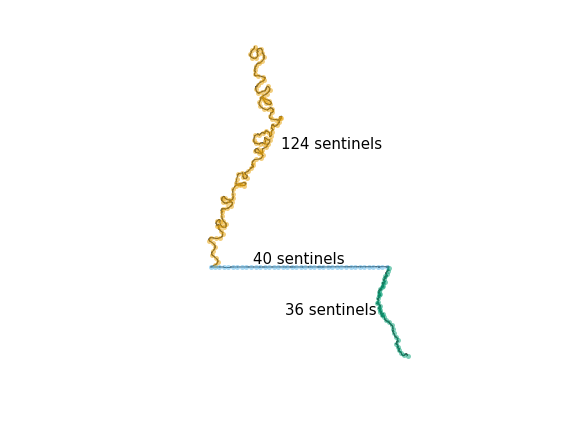
\includegraphics{../figures/mississippi_counts.png}
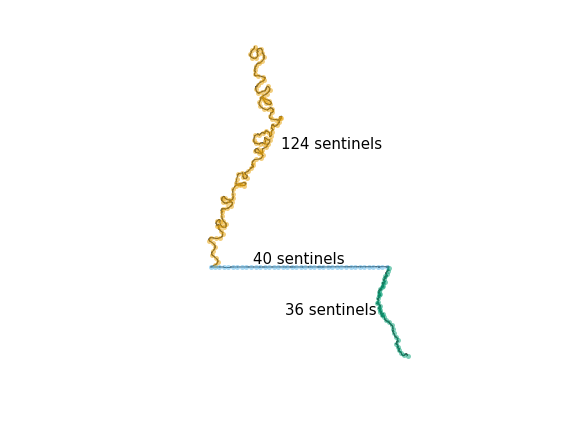
\includegraphics[height=0.5\textheight]{../figures/mississippi_counts.png}
\caption{\label{fig:mississippi_counts} 
Evenly spaced sentinels along the border between Mississippi and Louisiana.
From north to south, the border first follows the Mississippi river, becomes a straight line from west to east, and then follows the Pearl river.
Placing equispaced sentinels along the border results in the overrepresentation of the more sinuous sections of the border.
}
\end{figure}

The unweighted and density-weighted mean treatment estimands are both affected by the shape of the border between the treatment and control regions,
giving higher weight to wigglier sections of the border.
We illustrate this with the border separating two American States: Louisiana and Mississippi.
From North to South, the border follows the meandering Mississippi river, then takes a sharp turn to the East and becomes a straight line, until it meets the even more sinuous Pearl river, which it then follows until it reaches the Gulf of Mexico.
Sentinels placed at equal distance intervals along this border will therefore be more densely packed along the rivers, and sparsest along the straight segment (see Figure \ref{fig:mississippi_counts}).
When averaging a function over the border, those sections will therefore be overrepresented.
Troublingly, the sinuousness of the border therefore determines the estimand, even though the outcomes of interest will generally have nothing to do with river topologies.
In population terms, the result is that units near wigglier segments receive more weight.
Worse, the resolution of the map used in the analysis affects the estimated ATE.

This unwelcome dependence of the \(\unifavg\) estimand on the border topology is a symptom of the geometry of the problem: the 1-dimensional treatment function \(\tau(\border)\) is embedded in a Euclidean 2-dimensional space.
The dependencies induced by this geometric fact are reflected in the covariance \(\Sigma_{\sentinels \mid Y}\): sentinels in the straight segment of the border will be less strongly correlated than in the sinuous segments.
The more correlated sentinels individually carry less information about the local treatment effect.
Instead of averaging the posterior treatment effect along the border based on geometry or population, we consider averaging the information contained therein.
This motivates the inverse-variance weighted mean \(\invvar\):
\begin{equation}
\begin{split}
    \left. \invvar \mid Y, \hyperparam \right. &\sim \normal\del{\mu_{\invvar \mid Y}, \Sigma_{\invvar \mid Y}} ~ \text{, with} \\
    \mu_{\invvar \mid Y} &= \del{\ones\trans \Sigma_{\sentinels \mid Y}^{-1} \mu_{\sentinels \mid Y}} \big/ \del{\ones\trans \Sigma_{\sentinels \mid Y}^{-1} \ones} \,\textrm{, and} \\
    \Sigma_{\invvar \mid Y} &= 1 \big/ \del{\ones\trans \Sigma_{\sentinels \mid Y}^{-1} \ones} \,.
\end{split}
\eqlabel{eq:invvar}
\end{equation}
This estimator efficiently extracts the information from the posterior treatment effect, as it minimizes the posterior variance amongst weighted averages of the form \eqref{eq:weighted_estimand}.
It automatically gives more weight to sentinels in dense areas (as the variance will be lower there), and to sentinels in straight sections of the border (as the correlations between sentinels will be lower).

The estimand is still a weighted mean, with weights for the sentinels given by \(\weightb(\sentinels) = \Sigma_{\sentinels \mid Y}^{-1} \ones\).
This can put negative weights on some sentinels, as seen in a simulated example in Figure~\ref{fig:weight_functions}(c), and generally this estimand doesn't lend itself to an intuitive interpretation.
This estimand isn't chosen on scientific grounds, but rather it is dictated by the observed data.
This is counter to the conventional wisdom in causal inference, that the estimand should be chosen based on substantive grounds, ideally before collecting any data.
While perhaps unorthodox, analogous ``estimands of convenience'' have been proposed in other settings, for example matching methods that exclude some unmatched units from the analysis \citep[discussed in][]{crump2009dealing}, or in the context of balancing treatment and control populations with little overlap in their covariate distributions \citep{li2016balancing}.
The classical RDD could be said to provide another example, as the estimand \eqref{eq:rdd_univ_estimand} focuses on the treatment effect near the threshold not because those units are of particular substantive interest, but because the available data restricts estimation of the treatment effect elsewhere.
    


    	\hypertarget{projected-finite-population-ate}{%
\subsection{Projected Finite-Population ATE}\label{projected-finite-population-ate}}
    


\begin{figure}[tbp]
\centering
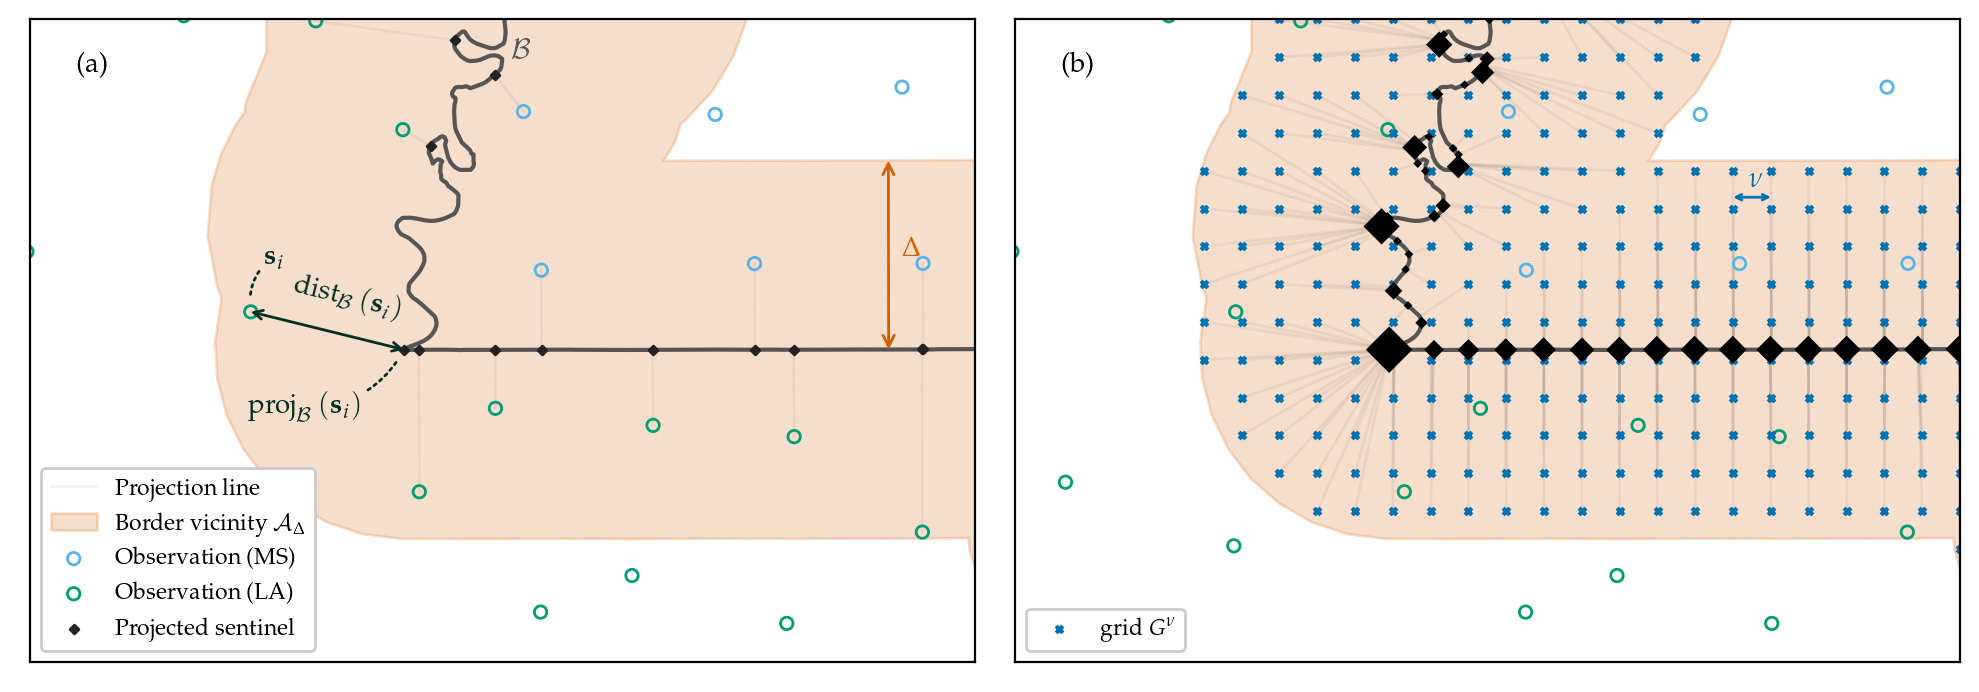
\includegraphics[width=\textwidth]{../figures/mississippi_projection_methods.png}
\caption{\label{fig:mississippi_projection_methods}
Illustration of (a) projected finite-population ATE \(\tauproj\), and (b) projected land ATE \(\taugeo\), using the border separating Mississippi and Louisiana near Baton Rouge, with units at the centroid of each county.
The border vicinity \(\area_\buffer\) is defined as all land within \(\buffer=50\,\mathrm{km}\) of the border.
With both methods, every projected sentinel has equal weight in the ATE, but the tight grid in (b) causes sentinels to coincide or nearly coincide, which we depict by scaling up the size of the marker by the number of coinciding sentinels.}
\end{figure}
    


    	All average treatment effect estimators considered so far presuppose evenly spaced sentinel points, which are then given weights.
Alternatively, we can project the positions of treatment and control units that are within a distance \(\buffer\) of the border onto the border, and use those projected sentinel positions without weights.
This is illustrated in Figure~\ref{fig:mississippi_projection_methods}(a).
For any point \(\svec\), we use the notation \(\proj_{\border}\del{\svec}\) to give the coordinates of the point on the border \(\border\) that is closest to \(\svec\) (assuming uniqueness), and \(\dist_{\border}\del{\svec}\) for the distance between the point and the border.
Let \(\vicinity{\svec}\) indicate inclusion in the border vicinity by returning one if \(\dist_{\border}\del{\svec} < \buffer\) and zero otherwise.
The projected finite-population \(\tauproj\) is then the uniformly weighted mean applied with the projected sentinels instead of the evenly spaced sentinels.
We can therefore modify \eqref{eq:unifavg}, replacing the cliff face mean vector \(\mu_{\sentinels \mid Y}\)
and covariance matrix \(\Sigma_{\sentinels \mid Y}\)
with equivalent quantities obtained at the projected sentinels,
to obtain the posterior mean and covariance of \(\tauproj\):
\begin{equation}\begin{split}
    \tauproj \mid \yt{}, \yc{}, \hyperparam &\sim \normal\del{\mu_{\tauproj \mid Y}, \Sigma_{\tauproj \mid Y}}\ \text{, with} \\
    \mu_{\tauproj \mid Y} &= 
    \frac{1}{
        \sum_{i=1}^{n_\treat{}+n_\ctrol{}}
        \vicinity{\svec_i}
    }
    \sum_{i=1}^{n_\treat{}+n_\ctrol{}}
        \vicinity{\svec_i}
        \E\sbr{
            \tau\del{
                \proj_{\border}\del{\svec_i}
            }
            \mid Y, \hyperparam
        } \ \text{, and}\\
    \Sigma_{\tauproj \mid Y} &= 
        \frac{1}{
            \del{
                        \sum_{i=1}^{n_\treat{}+n_\ctrol{}}
                        \vicinity{\svec_i}
            }^2
        }
        \sum_{i=1}^{n_\treat{}+n_\ctrol{}} 
        \sum_{j=1}^{n_\treat{}+n_\ctrol{}} 
        \vicinity{\svec_i}
        \vicinity{\svec_j}
        \cov\sbr{
            \tau\del{
                \proj_{\border}\del{\svec_i}
            },
            \tau\del{
                \proj_{\border}\del{\svec_j}
            }
            \mid Y, \hyperparam
        }\,.
\end{split}
\eqlabel{eq:tauproj}
\end{equation}
The posterior expectations and covariances in \eqref{eq:tauproj} can be obtained as in \eqref{eq:postvar2gp}, but using the projected sentinels.
Note that \(\tauproj\) is in the class of weighted mean estimands \eqref{eq:weighted_estimand},
with weight function \(\weightb(\sentinel) = \sum_{i=1}^{n_\treat{}+n_\ctrol{}} \vicinity{\svec_i} \delta\del{ \sentinel - \proj_\border(\svec_i)}\), where \(\delta\) is the Dirac delta function.

The resulting estimator has desirable properties: densely populated regions receive proportionately more sentinels, but wigglier segments of the border do not.
While it lacks the information efficiency of the inverse-variance estimator,
the projected estimand is easier to understand and interpret,
and may feel more familiar to practitioners used to finite-population inference.
The averaging is over the observed units, although with their locations projected to the border.

In our experience, the choice of \(\buffer\) does not have a large effect on the estimate yielded by \eqref{eq:tauproj}.
A reasonable heuristic is to set \(\buffer\) to a small multiple of the Gaussian process lengthscale \(\ell\).
It should be noted that this choice only affects the location of sentinels on the border, the Gaussian process always gives low unit weights \eqref{eq:unit_weights} to units far away from the border.
    


    	\hypertarget{projected-land-ate}{%
\subsection{Projected Land ATE}\label{projected-land-ate}}

In certain applications, population-based estimands can be undesirable, especially if the locations at which measurements are made are not representative of the population of interest.
In such cases, geography-weighted estimands can be more natural.
See \cite{antonelli2016positive} for a discussion of this distinction in the context of preferential sampling.
Remember that the ``geometry-based'' estimand \(\unifavg\) places uniform weights along the border.
Instead, the ``geography-based'' projected land ATE estimand \(\taugeo\), illustrated in Figure \ref{fig:mississippi_projection_methods}(b), begins by placing uniform weights on the treatment and control areas \(\area_\treat\) and \(\area_\ctrol\) that are within distance \(\buffer\) of the border \(\border\), but then projects them onto the border to derive border weights.
In other words, the projection method from \(\tauproj\) is applied to an infinite population of uniform density on both sides of the border, instead of the finite population of observed units.

We denote the border vicinity area by \(\area_\buffer\), defined as all points \(\svec\) such that \(\svec \in {\area_\treat \cup \area_\ctrol}\), and \(\dist_{\border}\del{\svec} < \buffer\).
To estimate \(\taugeo\), a tight grid \(\grid\) of evenly spaced points separated by \(\gridres\) is first generated covering \(\area_\buffer\).
Denote the number of grid points by \(L_\gridres\).
Each point \(\grid_l\), \(l=1,\dotsc,L_\gridres\) in \(\grid\) is then projected onto the border to become a sentinel.
The treatment effect at these positions is then estimated as before, yielding a mean vector and covariance matrix akin to \eqref{eq:postvar2gp}.
The mean of the mean vector then gives an estimate of \(\taugeo\).
In other words, \(\taugeo\) is estimated by applying the \(\unifavg\) procedure with sentinels obtained by projecting the grid points, instead of equispaced sentinels.
\(\taugeo\) remains in the category of weighted-mean estimands, with the weight function \(\weightb(\sentinel)\) in \eqref{eq:weighted_estimand} proportional to the area of \(\treatarea\) and \(\ctrolarea\) that \(\sentinel\) is nearest to, which can be written as the limit as the grid spacing goes to zero of point masses at the grid locations projected onto the border:
\begin{equation}
    \weightb(\sentinel) = \lim_{\gridres \rightarrow 0}\frac{1}{L_\gridres}\sum_{l=1}^{L_\gridres} \Ind\cbr{\sentinel = \proj_{\border}\del{\grid_l} }\,,
\end{equation}
where \(\Ind\) is the indicator function that returns one if its argument is true and zero otherwise.

For certain applications, it may be desirable to further restrict \(\area_\buffer\) to only certain types of land, for example residential areas in social studies, or farmland in agricultural studies.
However, it is important to note that \(\taugeo\) is never interpretable as the average treatment effect in the vicinity of the border, that is \(\taugeo \neq \int_{\area_\buffer} \tau(\svec) \dif \svec\).
Estimating the latter estimand would require predicting the conditional regression function at grod locations within the treatment or control region using only observations on the \emph{other} side of the border, which increases the extent of extrapolation required and thus makes the analysis more vulnerable to model misspecification.
    


    	\hypertarget{projected-super-population-ate}{%
\subsection{Projected Super-Population ATE}\label{projected-super-population-ate}}

Lastly, the purely geographical estimand \(\taugeo\) can be modified by weighting the grid points \(\grid_l\), \(l=1,\dotsc,L_\buffer\) by the population density \(\rho\del{\grid_l}\).
This gives the projected superpopulation ATE \(\taupop\).
Similarly to the density-weighted ATE \(\taurho\), estimating \(\taupop\) requires an estimate of the density \(\rho\del{\grid_l}\) at every grid point.
As before, the uncertainty in the estimate of \(\rho\) should in principle be propagated to the estimate of \(\taupop\), which generally will make the posterior distribution of \(\taupop\) neither normal nor analytically tractable.

The estimand \(\taupop\) can be interpreted as giving equal weight to each unit in the superpopulation of units within the border vicinity \(\area_\buffer\), but then moving each unit from its original location to its nearest location along the border, where the GeoRDD setting allows for the estimation of the treatment effect without undue extrapolation, and finally averaging the treatment effect of each unit in this displaced superpopulation.
    


    	\hypertarget{wiggly-border-simulation}{%
\subsection{Wiggly Border Simulation}\label{wiggly-border-simulation}}

\label{sec:wiggly_border}
    

\begin{figure}[tbp]
\centering
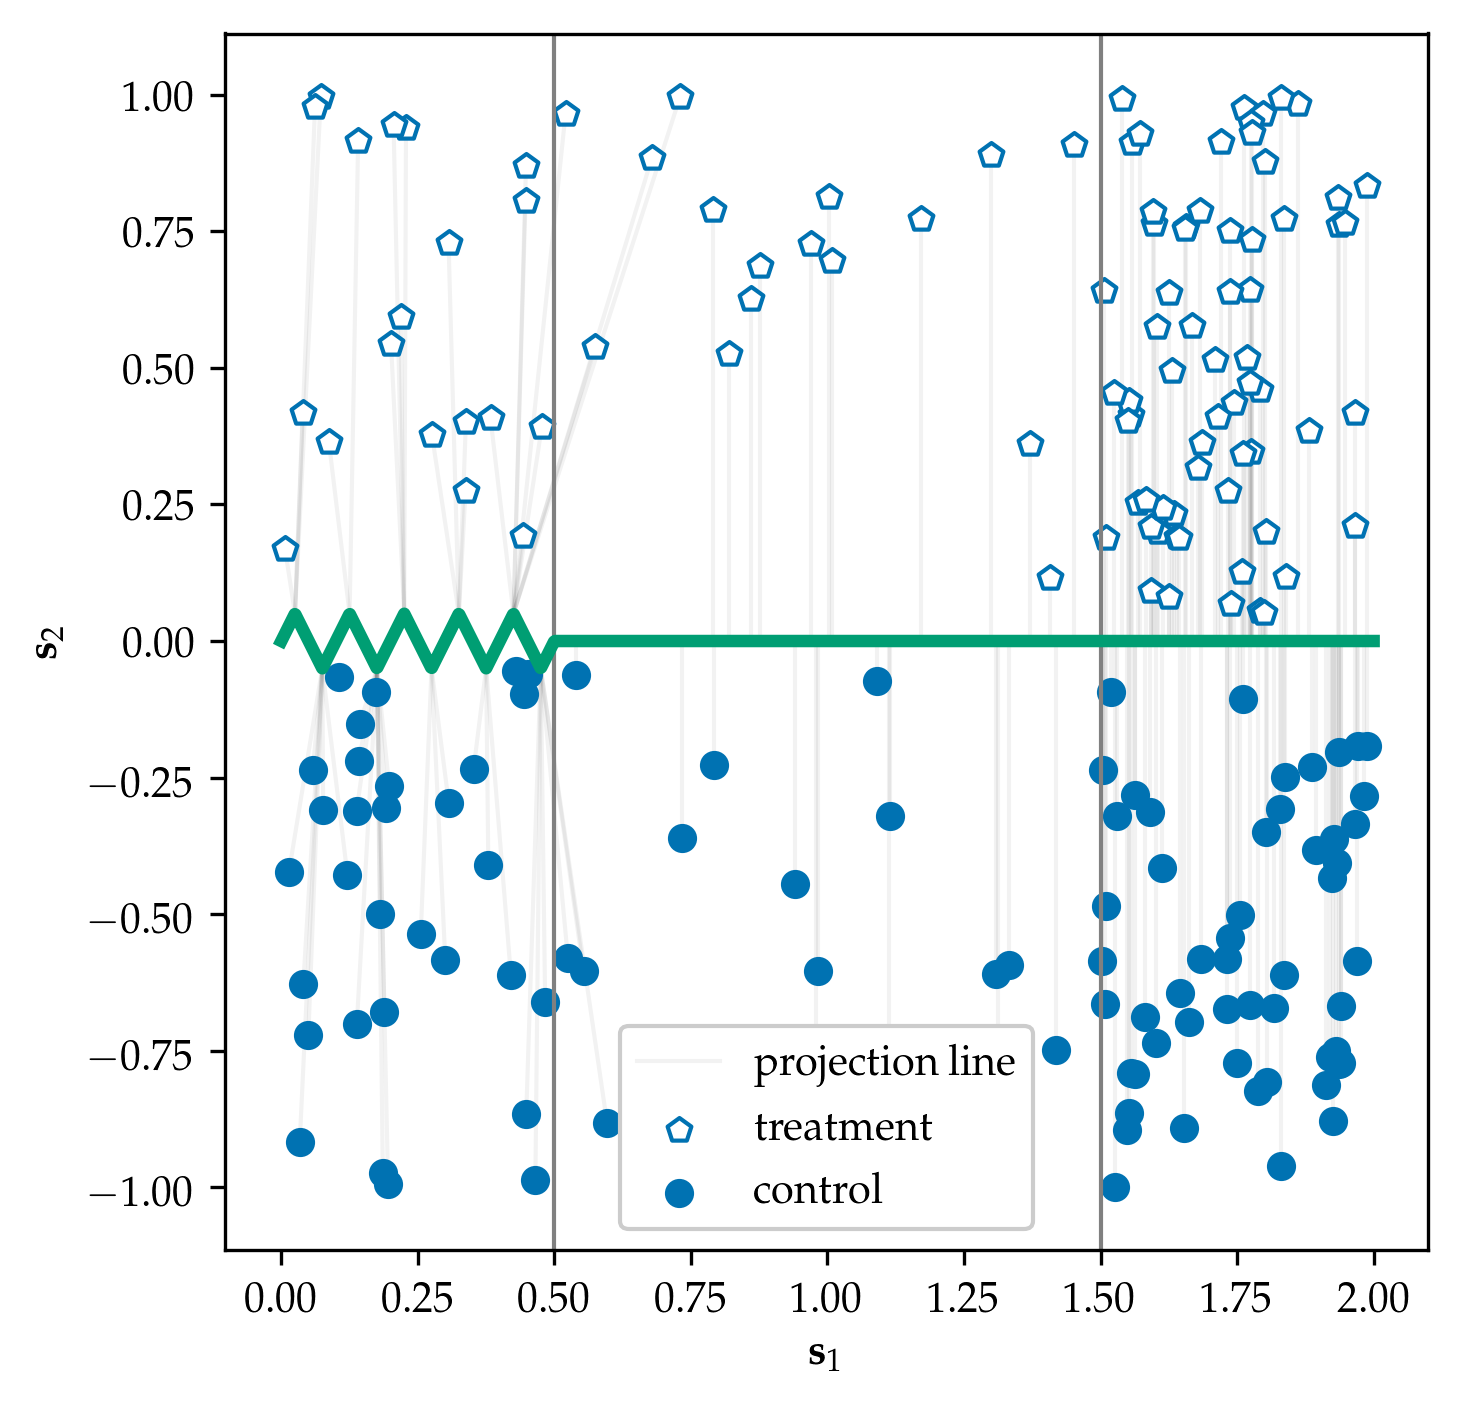
\includegraphics[height=0.35\textheight]{../figures/wiggly_boundaries_setup.png}
\caption{\label{fig:wiggly_boundaries_setup}Spatial positions of units and border for the wiggly border simulation of Section~\ref{sec:wiggly_border}. Projection lines for the projected finite population ATE are shown in light gray.}
\end{figure}
    

    	We illustrate the above ATE estimators with a simulation.
200 units are placed in a square area delimited by spatial coordinates \(S_1 \in \cbr{0,2}\) and \(S_2 \in \cbr{-1, 1}\).
A border at \(S_2=0\) divides units vertically into a control and treatment region,
which are then further divided horizontally at \(S_1=0.5\) and \(S_1=1.5\) into three bands:

\begin{itemize}
\tightlist
\item
  The leftmost band \(S_1 < 0.5\) has a weak treatment effect.
\item
  The middle band \(0.5 \ge S_1 < 1.5\) has a much lower population density, and a stronger treatment effect.
\item
  The rightmost band \(S_1 \ge 1.5\), has a much higher population density, and a very strong treatment effect.
\end{itemize}

Furthermore, the border in the leftmost band is a triangular wave, to create ``wiggliness.''
We increase the number of wiggles from 0 to 1000 to observe the effect on the estimates.
The simulation setting is summarized in Table~\ref{table:wiggly_setup}.
We draw a single set of spatial coordinates, shown in Figure~\ref{fig:wiggly_boundaries_setup}, then draw 10,000 simulations of the outcomes \(Y\) from a Gaussian process with squared exponential kernel (\(\ell=0.4\), \(\sigma=0.5\)).
To units above the border we add a treatment effect \(\tau(S_1, S_2) = S_1\).



\begin{table}[tbp]
\centering
\begin{tabular}{llll}
\hline
& Left \(S_1< 0.5\) & Middle \(0.5 \ge S_1 < 1.5\) & Right \(1.5 \ge S_1\)\tabularnewline
\hline
\textbf{Border} & wiggly & straight & straight\tabularnewline
\textbf{Density} & low \(\rho=1.0\) & very low \(\rho=0.3\) & high \(\rho=2.0\)\tabularnewline
\(\taubold\) & weak & medium & strong\tabularnewline
\hline
\end{tabular}
\caption{Summary of wiggly border simulation setup. \label{table:wiggly_setup}}
\end{table}

    	We fit the Gaussian process model \eqref{eq:spec2gp},
using the known hyperparameters of the covariance kernel and a weak prior on the mean parameter of each region,
and estimate the average treatment effect using the six methods proposed above.
In Figure \ref{fig:wiggly_boundaries_posteriors}(a) we show, for each estimator, the corresponding estimand and average posterior mean estimate evolving as the number of border wiggles increases.
The behavior of the posterior standard deviation is shown in Figure~\ref{fig:wiggly_boundaries_posteriors}(b).

\begin{figure}[tbp]
\centering
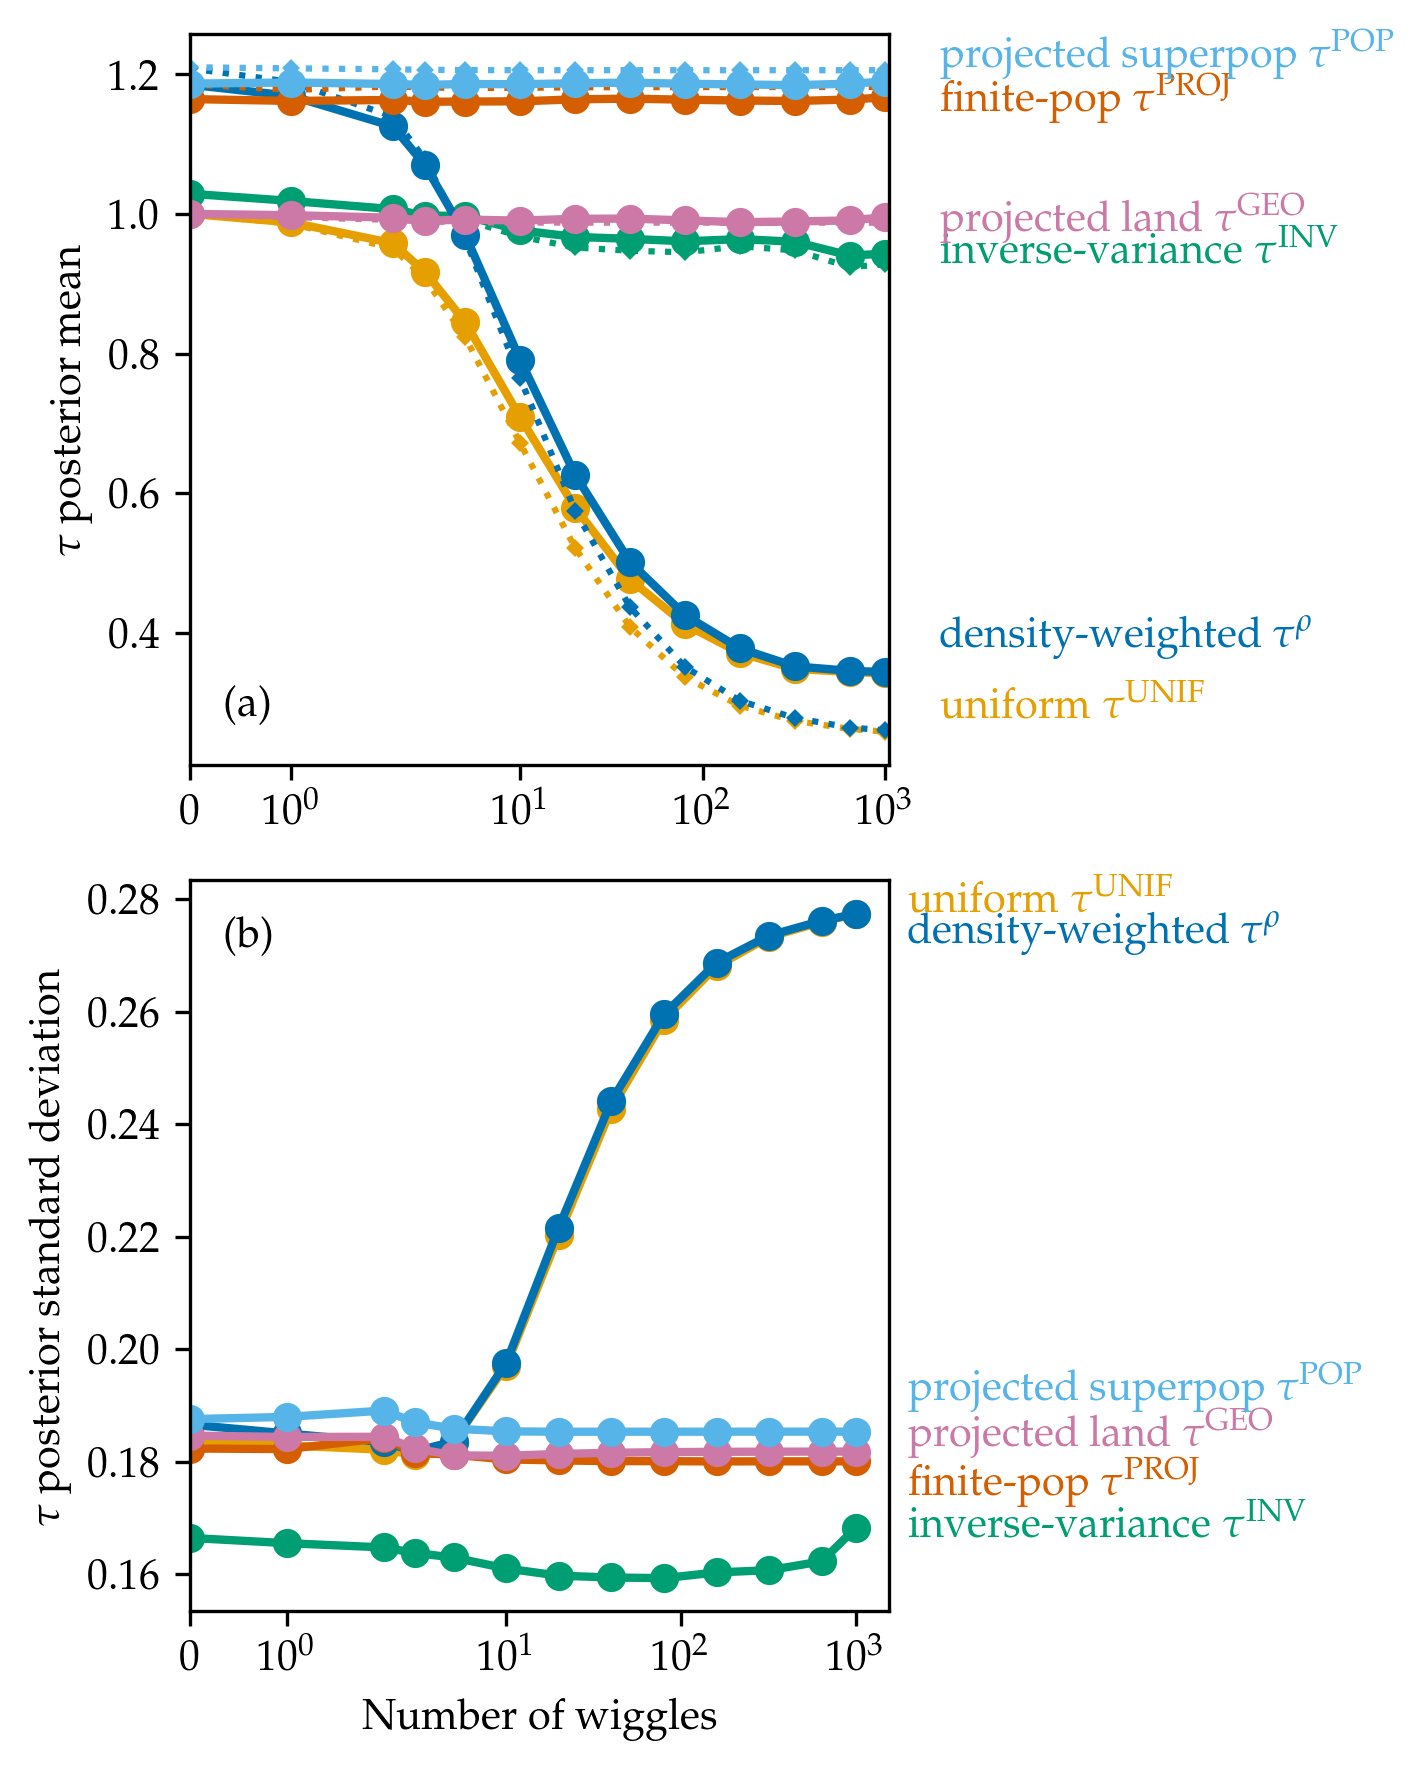
\includegraphics[height=0.4\textheight]{../figures/wiggly_boundaries_posteriors.png}
\caption{\label{fig:wiggly_boundaries_posteriors} Results of the simulations of Section~\ref{sec:wiggly_border}, showing for each ATE estimator as the leftmost section of the border gets wigglier (a) the estimate (posterior mean) averaged over 10,000 simulations with the corresponding estimand shown as a dotted line of the same color, and (b) the posterior standard deviation.}
\end{figure}
    
As the border is a straight line and \(\treatarea\) and \(\ctrolarea\) are rectangles,
and as the treatment effect does not depend on the vertical axis \(S_2\),
the density-weighted estimand \(\taurho\) equals the projected superpopulation estimand \(\taupop\),
and they are in fact both equal to the infinite-population average treatment effect.
Correspondingly, the posteriors of \(\taurho\) and \(\taupop\) are identical.
With 200 units, \(\taupop\) and the finite-population projected ATE \(\tauproj\) are also similar, but the latter has the advantage of not require estimating the population density.

The geometry- and geography-based ATE \(\unifavg\) and \(\taugeo\) are also equivalent when the border is a straight line.
They give equal weight to the sparsely populated middle band, which produces a lower estimate with higher variance than the posteriors of \(\taurho\) and \(\taupop\).

Lastly, the information-based inverse-variance estimand \(\invvar\) does not coincide with any others.
The estimand and mean estimate change slightly from 0 to 1 wiggles, but remains stable thereafter, demonstrating the robustness of this estimator to border topology.
Weighting by the inverse variance gives the lowest posterior variance within the class of ATEs under consideration, which can indeed be seen in Figure \ref{fig:wiggly_boundaries_posteriors}(b).

As we introduce wiggles into the leftmost band,
\(\taurho\) and \(\unifavg\) show their susceptibility to the border topology.
Proportionally more sentinels are packed into the leftmost section of the border,
upweighting the lower treatment effect of that band,
and resulting in a drop of the two estimates and estimands.
Meanwhile, \(\invvar\) remains stable despite the wiggles,
because the additional sentinels in the leftmost
band get automatically downweighted as their correlation rises.
The estimators that rely on projection
\(\tauproj\), \(\taugeo\), and \(\taupop\) also remain stable,
because the projected sentinels hardly move.
These robust estimands show only a slight displacement when the first wiggles are introduced,
caused by the presence of some sentinels nearer to the observed units.
    
\begin{figure}[ptb]
\centering
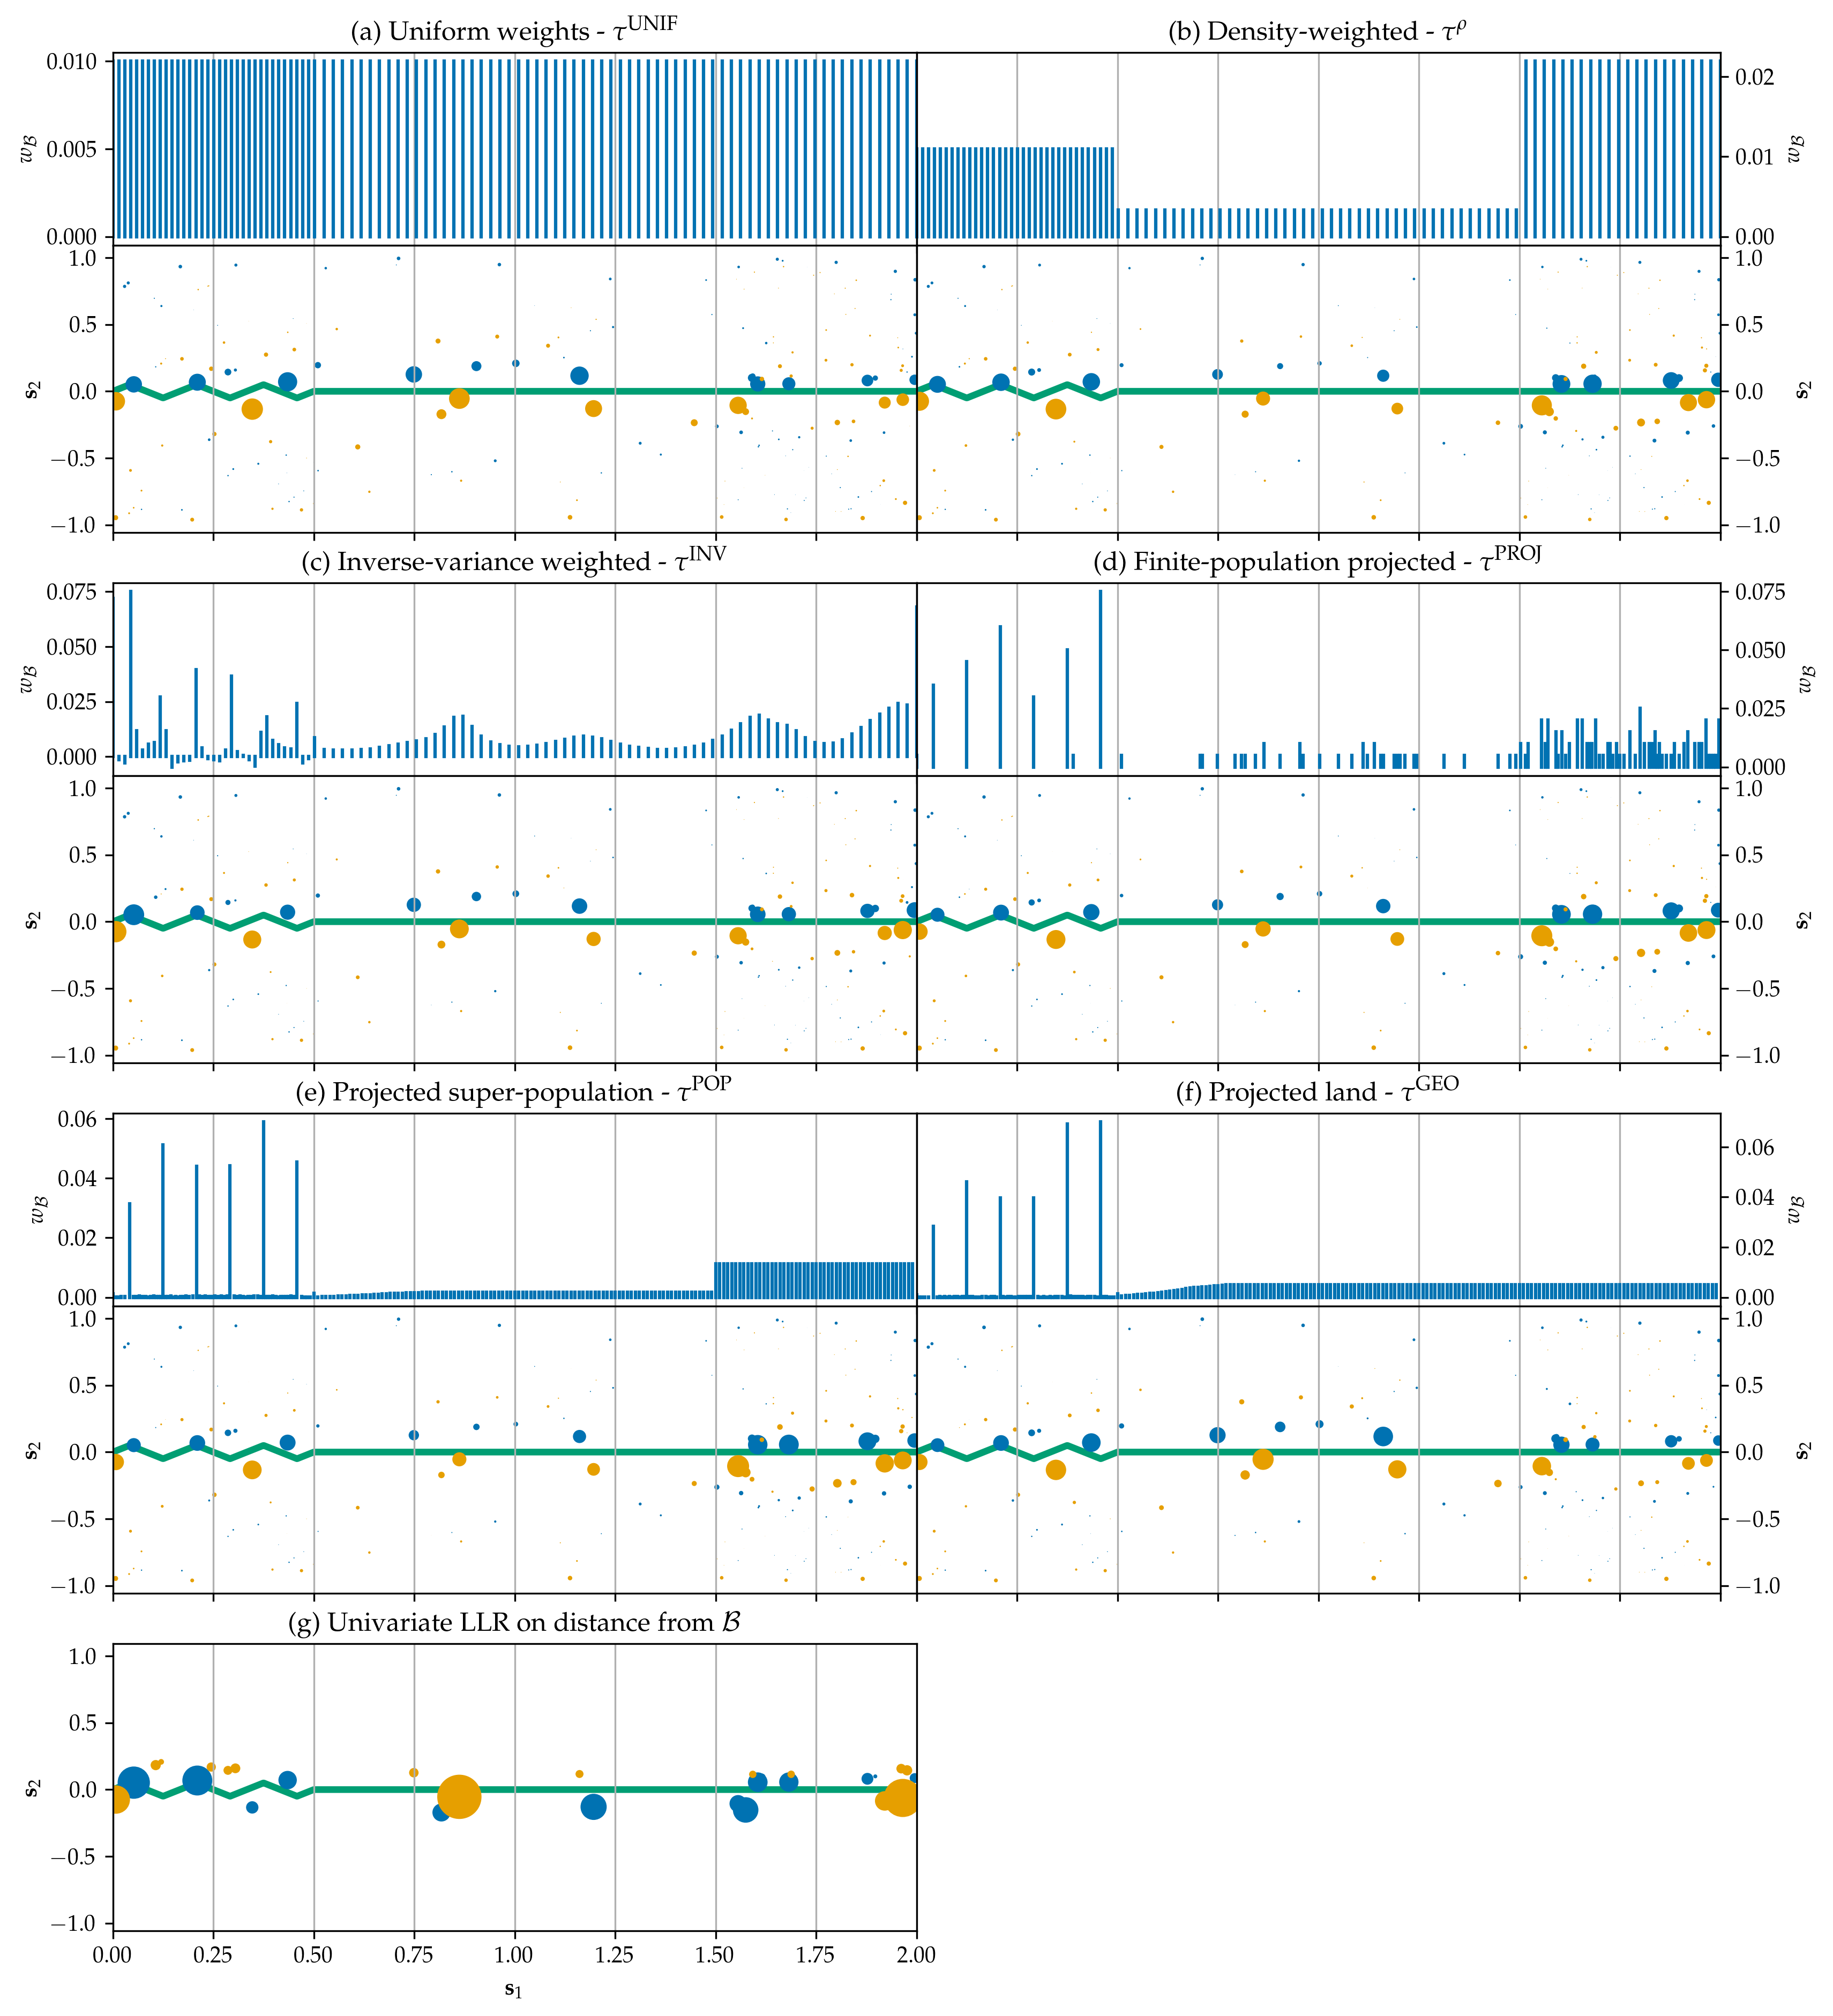
\includegraphics[width=\textwidth]{../figures/weight_functions.png}
\caption{\label{fig:weight_functions}Weight functions and induced weights on the observations for the six weight functions proposed in this paper. The weight function plots show the weight \(\weightb(\sentinel)\) against each sentinel's \(S_1\) coordinate. Sentinels with coinciding or nearly coinciding (within 0.005 of each other) coordinate \(S_1\) were merged and their weights summed. The induced weight plots show a circle for each unit, with the area of the circle proportional to its weight (\(\wt\) and \(\wc\) for treatment and control units respectively), and colored in blue for positive weights and orange for negative weights.}
\end{figure}
    

    	In Figure~\ref{fig:weight_functions}(a-f), we illustrate the behavior of border weights \(\weightb(\sentinel)\) and unit weights (\(\wt\) and \(\wc\)) in this simulation setting with 3 wiggles.
Note how evenly spaced sentinels (for \(\unifavg\), \(\taurho\), and \(\invvar\)) are more densely packed along \(S_1\) in the leftmost area because of the zig-zagging border.
The inverse-variance weighted estimator border weights can be seen to respond to this change in the border topology, though it is difficult to interpret their oscillating behavior.
While these border-weights look unreasonable and unstable, the induced unit weights for \(\invvar\) are well-behaved, and in fact quite similar to those of the projected finite- and infinite-population estimators.
Furthermore, note that all estimators can give some small negative weights \(\wt\) to treatment units, and small positive weights \(\wc\) to control units.
For Gaussian processes, this can be understood in terms of the negative side-lobes of the equivalent kernel (see \cite{rasmussen2006gaussian} Section 2.6).
The high variance of \(\unifavg\) and \(\taugeo\) manifests itself as large weights given to a small number of units.
All other estimators spread the weights more evenly amongst the units near the border, which reduces their variance.
    


    	For comparison, the weights placed on units by the projected 1D RDD are shown in Figure~\ref{fig:weight_functions}(g).
A triangular kernel in \(S_2\) was used with bandwidth selected using the MSE-minimizing method proposed by \cite{imbens2012optimal}.
The Projected 1D~RDD estimator can also be written as a linear combination of the observed outcomes \eqref{eq:unit_weights}, and the unit weight vectors can be derived as:
\begin{equation}
\begin{split}
\wt &= \hphantom{-} \Xmat_b (\Xmat_\treat\trans \Wmat_\treat \Xmat_\treat)^{-1} \Xmat_\treat\trans \Wmat_\treat \,, 
\text{ and}
\\
\wc &= - \Xmat_b (\Xmat_\ctrol\trans \Wmat_\ctrol \Xmat_\ctrol)^{-1} \Xmat_\ctrol\trans \Wmat_\ctrol \,, 
\end{split}
\eqlabel{eq:unit_weights_llr}
\end{equation}
where \(\Xmat_b = \del{1~0}\), \(\Xmat_\treat\) is the \(n_\treat \times 2\) design matrix with the first column filled with ones and the second column containing the distance from the border of each treatment unit, and \(\Wmat_\treat\) is an \(n_\treat \times n_\treat\) diagonal matrix where the \(i^\mathrm{th}\) diagonal element is the triangular kernel evaluated on the \(i^\mathrm{th}\) unit's distance from the border.
The \(\Xmat_\ctrol\) and \(\Wmat_\ctrol\) matrices are analogously defined for control units.
By construction, the unit weights drop to zero outside of the support of the kernel.
Within the support, Projected 1D RDD can also give negative weights to treatment units, and positive weights to control units.
This results from the negative influence on the prediction \(\widehat{y^*}\) at \(x^*\) that univariate linear regression can give to an observation \(Y_i\) at \(X_i\) sufficiently far away on the opposite side of the mean \(\overline{X}\) of all observations.
Strikingly, almost all of the positive weights are given to units in the rightmost treatment area that are closest to the border, and almost all the negative weights are given to units in the leftmost control area.
Consequently, any trend in the outcomes across \(S_1\) would confound the estimated treatment effect.

In most applications, we recommend the use of the finite population or inverse-variance-weighted estimators, to prevent the undesirable influence of border topology.
The projected finite population method is simplest to understand and interpret in the tradition of finite population estimators, and unlike the projected superpopulation estimator \(\taupop\) it does not require estimating population density.
Meanwhile, the inverse-variance estimator is the most efficient (lowest posterior variance) weighted mean estimator,
and avoids the potential complication of the choice of a distance cutoff for projected units.
    

\begin{table}[tbp]
\centering
\begin{tabular}{llllll}
\hline
Symbol     & Description                     & $\border$ Topology & Sentinels       & Principle         & Variance \\
\hline
$\unifavg$ & Uniform ATE                     & Sensitive       & Equispaced      & Geometry    & High     \\
$\taurho$  & Density-weighted ATE            & Sensitive       & Equispaced      & Population  & Low      \\
$\invvar$  & Inverse-var. weighted ATE   & Robust          & Equispaced      & Information & Lowest   \\
$\tauproj$ & Projected finite pop. ATE & Robust          & Projected Units & Finite-pop. & Low      \\
$\taugeo$  & Projected land ATE              & Robust          & Projected Grid  & Geography   & High     \\
$\taupop$  & Projected superpop. ATE   & Robust          & Projected Grid  & Population  & Low \\
\hline
\end{tabular}
\caption{Summary of average treatment effect estimtor and estimand properties.}
\label{table:estimator_properties}
\end{table}
    	\hypertarget{testing-for-non-zero-effect}{%
\section{Testing for Non-Zero Effect}\label{testing-for-non-zero-effect}}
    

\label{sec:hypothesis_testing}
    	Once we have obtained the ``cliff face'' estimate \eqref{eq:postvar2gp} and estimated an average treatment effect, we might also naturally wonder whether we can claim to have detected a significant treatment effect at the border.
In the hypothesis testing framework, we have two possible choices of null hypotheses.
The \textbf{sharp null} specifies that the treatment effect is zero everywhere along the border:
\(\tau(\border)=0\),
while the \textbf{weak null} only requires the average treatment effect to be zero.
    


    	\hypertarget{marginal-likelihood-test}{%
\subsection{Marginal Likelihood Test}\label{marginal-likelihood-test}}

To target the sharp null hypothesis, we first define a parametric null model \(\modnull\),
specified as a single Gaussian process spanning the control and treatment regions,
with the same kernel and hyperparameters obtained in the 2GP procedure.
\(\modnull\) is smooth and continuous at the border,
and therefore accords with the sharp null hypothesis.
Intuitively, if there is a treatment effect,
the likelihood of the observations should be lower under \(\modnull\) than under \(\modalt\),
the 2\(\gp\) model as specified in equation \eqref{eq:spec2gp}.
We therefore choose the difference in log-likelihoods as our test statistic
\begin{equation}
    t = \log \Pr\del{\yt{}, \yc{} \mid \modalt} - \log \Pr\del{\yt{}, \yc{} \mid \modnull} \,,
\end{equation}
and wish to reject the sharp null hypothesis when its observed value \(t_{obs}\) is high.

A parametric bootstrap approach is used to quantify what ``high'' means. We draw \(\yt{}^*,\yc{}^*\) from \(\modnull\),
using the same spatial locations as in the original data,
and then fit the two competing models to the simulated data in order to obtain the bootstrapped test statistic
\begin{equation}
    t^* = \log \Pr\del{\yt{}^*, \yc{}^* \mid \modalt} - \log \Pr\del{\yt{}^*, \yc{}^* \mid \modnull}\,.
\end{equation}
Repeating this procedure, we obtain a distribution of \(t\) under \(\modnull\),
which we can then compare to the observed \(t\).
More precisely, we can interpret the proportion of \(t^*\) drawn above \(t_{obs}\) as a \(p\)-value
\begin{equation}
    p^{\mathrm{lik}} = \Pr\del{t^* > t_{obs} \mid \modnull}\,.
\end{equation}
Computationally, because the hyperparameters and locations of the units are held constant during the bootstrap, we can reuse the Cholesky decomposition of the covariance matrix, allowing the test to be performed in seconds even with hundreds of units and thousands of bootstrap samples.
    


    	\hypertarget{chi-squared-test}{%
\subsection{``Chi-squared'' Test}\label{chi-squared-test}}

The likelihood-based sharp null above is valid and easy to understand.
But it may seem odd that the test aims to detect a non-zero treatment effect at the border, without any explicit reference to the border \(\border\).
The test statistic and \(p\)-values can be computed without access to the sentinel positions, using only the treatment and control indicators.
If the test is significant, there is no guarantee that this is due to a discontinuity at the border.

To address this oddity, we can derive a test statistic directly from the cliff face estimator \eqref{eq:postvar2gp}.
We will use \(\muvec\) and \(\SigmaMat\) as shorthand for the posterior mean \(\muvec_{\sentinels \mid Y}\)
and covariance matrix \(\SigmaMat_{\sentinels \mid Y}\) throughout this section.
If a \(k\)-vector \(\yvec\) is distributed \(\normal\del{\muvec, \Sigma}\), with mean vector \(\muvec\) unknown and covariance \(\SigmaMat\) known, then under the null hypothesis that \(\mu=0\), the test statistic \(\yvec\trans \SigmaMat^{-1} \yvec\) has distribution \(\chi^2_k\).
See for example \cite{rencher2003methods} Section 5.2.2 for a classical derivation of this test.
This suggests that we could use \(S^2=\muvec\trans \SigmaMat^{-1} \muvec\) as a test statistic,
and obtain a \(p\)-value from a \(\chi^2_\numsent\) distribution function evaluated at \(S^2\), where \(\numsent\) is the number of sentinels.
However, we face two problems.
Firstly, this test, obtained heuristically from a Bayesian posterior by analogy with the classical multivariate normal result, is not a valid frequentist test.
Secondly, while \(\SigmaMat\) is mathematically full-rank, it is typically numerically rank-deficient.
Therefore, \(\numsent\) overestimates the true degrees of freedom of the null distribution.

Benavoli and Mangili (2015), developing a test for function equality, address the second problem by trimming the \(\SigmaMat\) eigenvalues \(\lambda_i\) lower than \(\epsilon \sum_{j=1}^k \lambda_j\), with \(\epsilon\) a pre-specified small number (they use 0.01).
They address the first problem by showing that the resulting \(p\)-value is always conservative in their simulations.
However, in our work, we found the resulting \(p\)-value to be sensitive to the arbitrarily chosen \(\epsilon\) tolerance parameter, which makes it difficult to trust its validity.

We therefore again take the parametric bootstrap approach, this time using \(S^2\) as the test statistic instead of the likelihood ratio.
With B bootstrap samples, the \(p\)-value is obtained as
\begin{equation}
\begin{split}
    p &= \frac{1}{B} \sum_{t=1}^T \Ind\cbr{S_{(b)}^2 < S^2}\  \text{, with}\\
    S_{(b)}^2 &= (\muvec_{(b)} )\trans \SigmaMat^{-1} \muvec_{(b)}\,,
\end{split}
\end{equation}
where \(\muvec_{(b)}\) is the result of applying \eqref{eq:postvar2gp} to \(\yt^{(b)}\) and \(\yc^{(b)}\), themselves drawn from \(\modnull\) at the same locations as the observations \(\yt\) and \(\yc\).

Because calculating \(S^2\) involves inverting a matrix \(\Sigma\) that is mathematically of full rank, but numerically of low rank, we may worry about the numerical stability of computing \(S\).
We verified in simulated examples that regularizing \(\Sigma\) by adding a small constant to its diagonal does not greatly affect the computed \(S^2\).
The parametric bootstrap ensures the frequentist validity of the test
regardless of the regularization.
    


    	\hypertarget{inverse-variance-weighted-test}{%
\subsection{Inverse-Variance Weighted Test}\label{inverse-variance-weighted-test}}

We now turn to the weak null hypothesis that the average treatment effect along the border is zero, but otherwise allowing the treatment effect to be positive along some parts of the border and negative in others.
As we saw in Section~\ref{sec:ate}, the ``average'' treatment effect can be defined in multiple ways.
If we choose the inverse-variance weighted mean, then \(\invvar\) has posterior given by \eqref{eq:invvar}.
While the posterior is a Bayesian object, we can use it heuristically to derive a pseudo-\(p\)-value:
\begin{equation}
\begin{split}
    Z_0 &\sim \normal\del{0, \Sigma_{\invvar \mid Y}} \,, \\
    p^{\mathrm{INV}} &= \Pr\del{ 
        \abs{Z_0} > 
        \abs{
            \mu_{
                \invvar \mid Y
            }
        } 
    } \\
    &= 2\Phi\del{-
        \frac{
            \abs{
                \mu_{
                    \invvar \mid Y
                }
            }
        }{
            \sqrt{
                \Sigma_{\invvar \mid Y}
            }
        }
    } \,.
\end{split}
\end{equation}
This ``\(p\)-value'' obtained from the Bayesian posterior may not have good frequentist properties.
In particular, there is no guarantee that under the null hypothesis, \(p^{\mathrm{INV}}\) is below 0.05 less than 5\% of the time.
To turn it into a valid frequentist test, it can be calibrated using the same parametric bootstrap approach that was used for the likelihood and \(\chi^2\) tests, now using \(\mu_{\invvar \mid Y}\) as the test statistic.
The calibration can also be achieved analytically, since \(\mu_{\invvar \mid Y}\) is normally distributed under the null hypothesis.
We derive the analytical calibration of the inverse-variance test in Appendix \ref{sec:calibration}.
Note that the \(p\)-value for all three tests defined in this section is derived under the same parametric null model \(\modnull\), which accords with both the sharp null and weak null hypotheses.
The calibrated inverse-variance test targets the weak null hypothesis in the sense that the test statistic is an estimate of the ATE (and thus the test is sensitive to deviations of the ATE from zero) rather than its \(p\)-value being derived under the weak null (like the classical \(t\)-test for example).

\label{eq:calib_test}
    


    	\hypertarget{power-in-simulated-example}{%
\subsection{Power in Simulated Example}\label{power-in-simulated-example}}

\label{sec:powersim}
    


\begin{figure}[tbp]
\centering
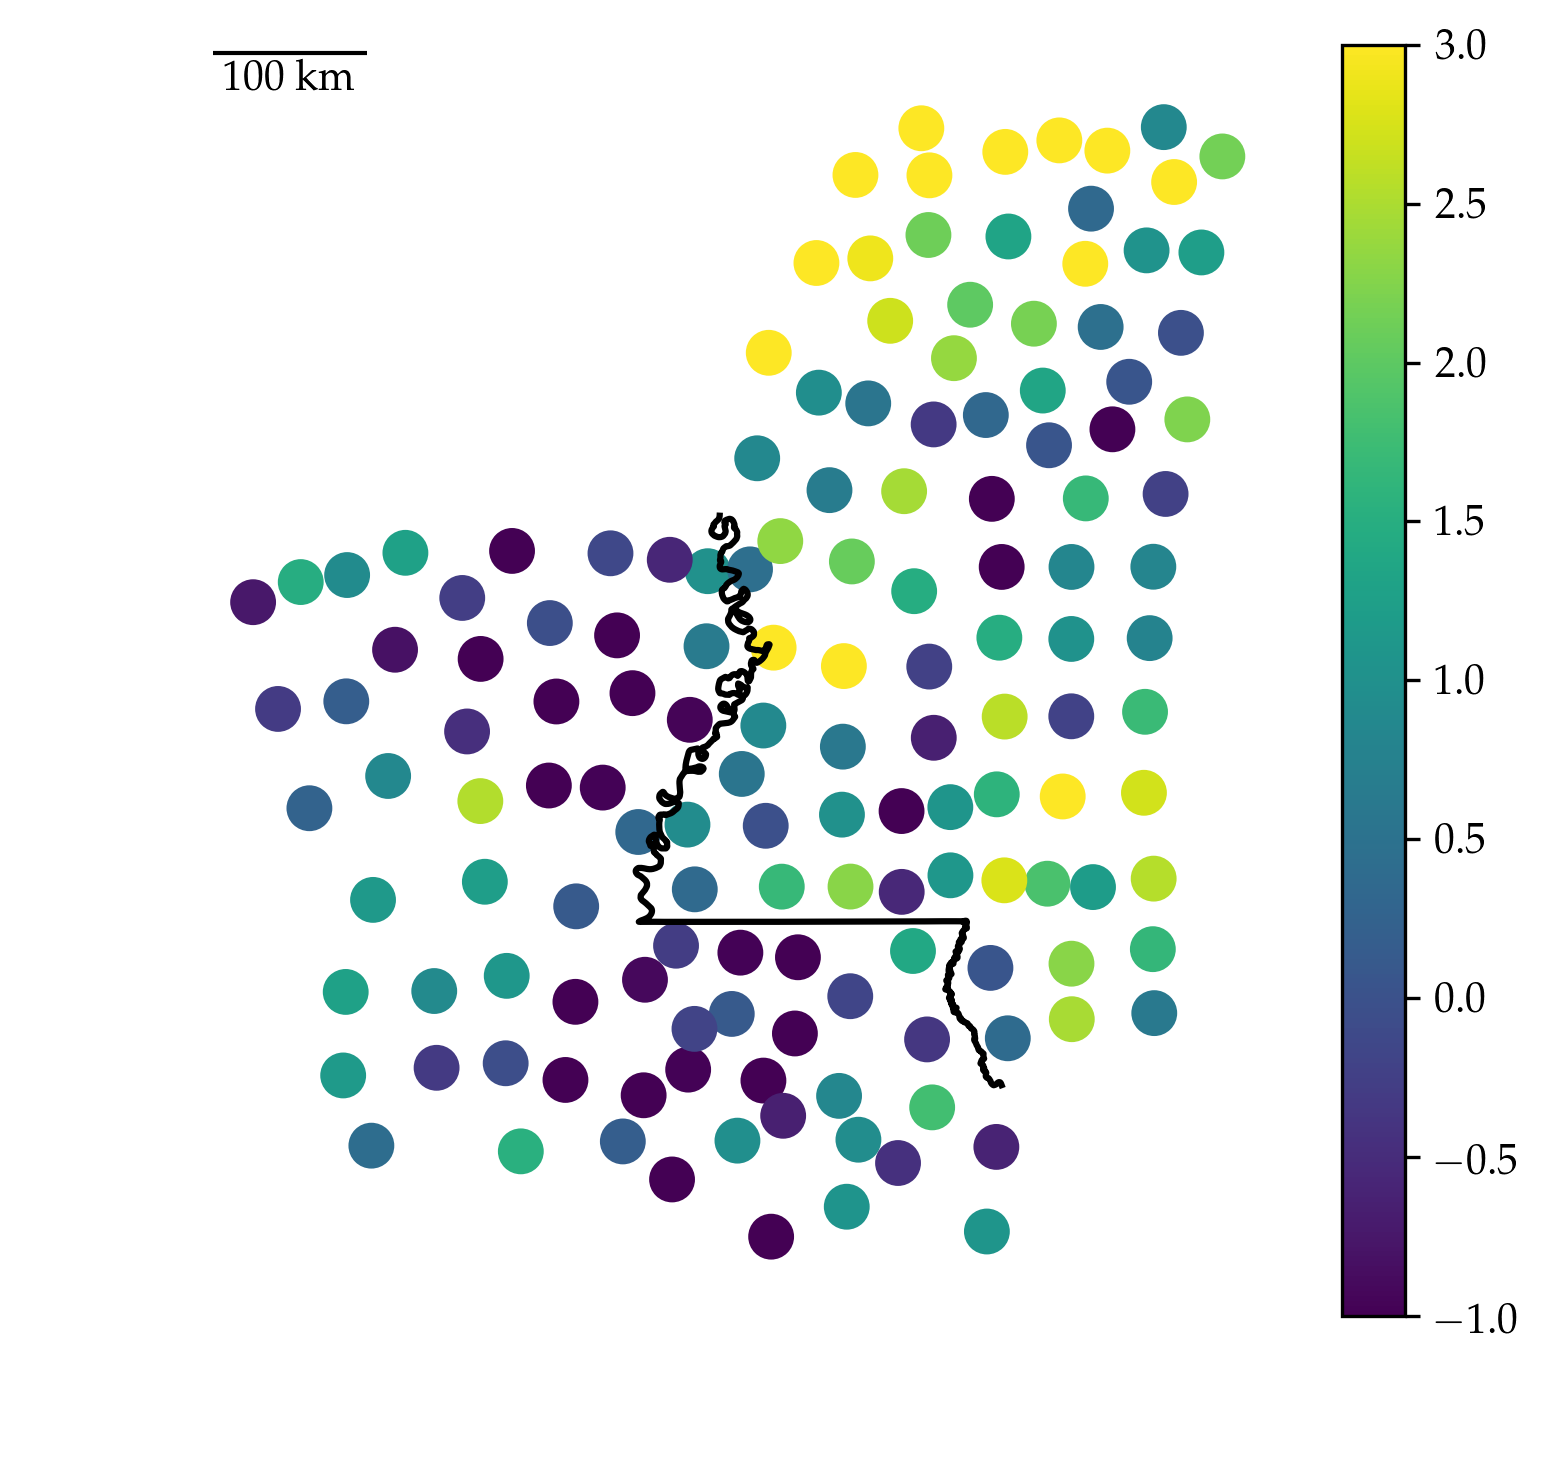
\includegraphics[height=0.4\textheight]{../figures/mississippi_sim.png}
\caption{\label{fig:mississippi_counties}Set-up of the imaginary experiment in Louisiana and Mississippi. Each unit is at the centroid of a county. The colors indicated the observed outcomes in one draw of the simulation under \(\tau=1.5\). In this particular run, the p-values were 0.0016, 0.0018, and 0.0013 for the mLL, \(\chi^2\), and inverse-variance test respectively.}
\end{figure}
    


    	The three tests we developed leverage different aspects of the problem, and target two different null hypotheses. One may wonder how their power compares in the presence of a treatment effect. Considering once more the border between Louisiana and Mississippi, we imagine an experiment where the unit of analysis is the county, located at its centroid, as shown in Figure \ref{fig:mississippi_counties}.
We will simulate outcomes from a single Gaussian process covering both states. For simplicity, we fix the hyperparameters to arbitrary values: \(\sigman=\sigmaf=1.0\) and \(\ell=100\,\mathrm{km}\).
We then add a constant treatment effect \(\tau\) to all the outcomes in Louisiana.
The results of the three tests proposed so far are shown in the first three rows of Table~\ref{table:power} for \(\tau=0\) (null hypothesis) and \(\tau=1.2\) and significance level \(\alpha=0.05\).
    

\begin{table}
    \label{table:power}
    \centering
    \begin{tabular}{rrr}
        \toprule
        & \multicolumn{2}{c}{Power under} \\
        Test & $\tau=0$ & $\tau=1.2$ \\
        \midrule
	    Marginal log-likelihood $ $ & 0.048 & 0.656 \\
	    $\chi^2$ & 0.047 & 0.635 \\
	    Inverse-variance $\Sigma^{-1}$ & 0.085 & 0.866 \\
	    Bootstrap-calibrated $\Sigma^{-1}$ & 0.050 & 0.799 \\
	    Analytically calibrated $\Sigma^{-1}$ & 0.051 & 0.801 \\
        \bottomrule
    \end{tabular}
    \caption{Power of marginal likelihood, chi-squared, and inverse-variance tests, with nominal significance of $\alpha=0.05$, under null and alternative hypothesis for simulated outcomes at the centroids of Louisiana and Mississippi counties.}
\end{table}
    	We see that under the null, the \(\chi^2\) and likelihood ratio tests are valid (rejection of the null in 5\% of simulations up to simulation error).
This is enforced by the parametric bootstrap, which draws test statistics from the same null distribution to calibrate the tests.
However, the \(p\)-values for the inverse-variance test are biased down, so that we will falsely reject the null \(6.7\%\) instead of \(5\%\) of the time.
While unfortunate, this is unsurprising, since the inverse-variance test was derived heuristically rather than from a rigorous frequentist procedure.

After calibration, the hypothesis test based on the inverse-variance mean is valid, but retains higher power to detect the constant treatment effect than the mLL and \(\chi^2\) tests.
This can lead to a paradox: we may reject the weak null hypothesis, but fail to reject the sharp null hypothesis (using the \(\chi^2\) or likelihood test), even though rejection of the weak null logically implies rejection of the sharp null.
This paradox isn't specific to this setting, and is discussed in depth in the context of randomization-based inference by \cite{Ding:2014sf}.
To maximize power, we therefore recommend using the calibrated inverse-variance test in studies where the main interest is in the detection of an overall (average) increase or decrease in outcomes.
    


    	\hypertarget{placebo-tests}{%
\subsection{Placebo Tests}\label{placebo-tests}}
    

\label{sec:placebo}
    	Gaussian process models are almost always misspecified.
We do not believe that the Gaussian process with stationary squared exponential kernel is the true data-generating process, although we hope that the model is sufficiently flexible to represent reality well.
Under misspecification, we should be skeptical of results that rely on the truth of the model specification.
We therefore encourage practitioners to probe the validity of the above hypothesis tests by running a ``placebo'' test.
A placebo test repeatedly applies the hypothesis test on data that are known to have zero treatment effect (a ``placebo''),
in order to verify that the returned p-values are uniformly distributed.
In our spatial setting, we will use the treatment and control regions separately as placebo groups.
Within each placebo group, we repeatedly draw an arbitrary geographical border, creating new treatment and control groups.
Here we drew lines that split the placebo units in half at a sequence of angles \(1\degree,2\degree,3\degree,\dotsc,180\degree\) counter-clockwise from horizontal, each positioned so that half of the units fall on either side of the line in order to maximize power.
Because the border was chosen arbitrarily by us, we should not expect there to be a discontinuous jump in outcomes at this border.
We then apply the bootstrapped likelihood test procedure described above to this arbitrarily divided data, store the results, and hope to obtain a roughly uniform distribution of p-values.
The resulting p-values will obviously be highly correlated, so we should only expect a very roughly uniform distribution (because of the small effective sample size), but at the very least, this procedure allows us to visually verify that the p-values are not blatantly biased.
    


    	\hypertarget{example-nyc-school-districts}{%
\section{Application: NYC School Districts}\label{application-nyc-school-districts}}

\label{sec:NYC_example}

We illustrate the analysis of geographical regression discontinuity designs using house sales data from New York City.
The city publishes information pertaining to property sales within the city in the last 12 months on a rolling basis.
This includes the sale price, building class, and the address of the property.
Public schools in the city are all part of the City School District of the City of New York, but the city-wide district is itself divided into 32 sub-districts.
It is a common belief that school districts have an impact on real estate price, as parents are willing to pay more to live in districts with better schools.
We therefore ask: can we measure a discontinuous jump in house prices across the borders separating school districts?
    


    	\hypertarget{preprocessing}{%
\subsection{Preprocessing}\label{preprocessing}}

In order to model the property sale prices, we need to obtain their locations.
We geocode the address of each sale by merging the sales with NYC's Pluto database, which contains X and Y coordinates for each house, identified by its borough, zip code, block and lot.
These coordinates are given in the EPSG:2263 projection in units of feet, which we also adopt.
For addresses that do not find a match in Pluto, we use Google's geocoding API to obtain a latitude and longitude, which we then project to EPSG:2263.

We then filter the sales data, by removing sales (1) without a reported sale price, (2) outside of the family homes building class categories (one, two, and three family dwellings); (3) missing the square footage or other covariates; (3) without a location due to failed geocoding; (4) smaller than 100 sq ft, and (5) outliers with log price per square foot less than 3 or more than 8.
We exclude condos and coops because only very few sales report square footage alongside the price.

We display the resulting dataset of 19,578 sales recorded between January 8, 2015 and December 7, 2016 in Figure~\ref{fig:sales_map}.
We also show the 27,394 residential properties that have missing square footage information.
Properties with missing square footage are almost all coops and condos, which explains the clustering of missing data in areas of higher density.
    


\begin{figure}[tbp]
\centering
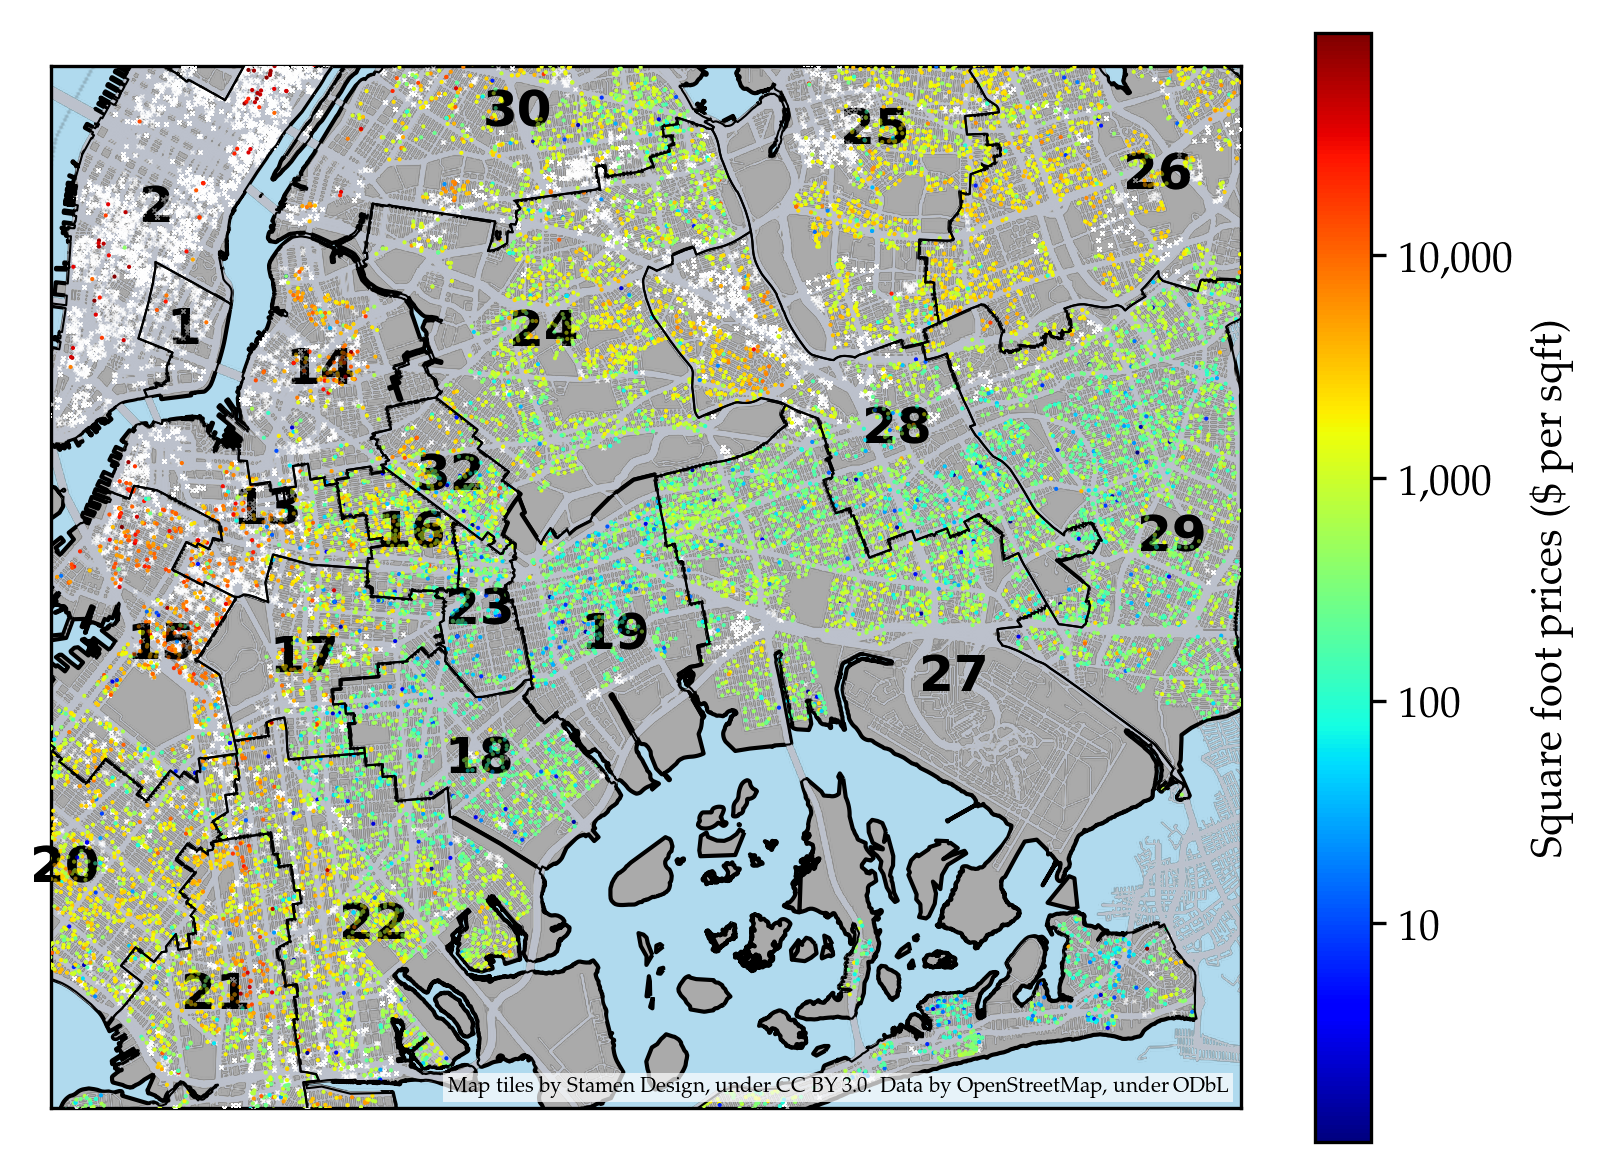
\includegraphics[width=\textwidth,height=0.4\textheight,keepaspectratio]{../NYC/NYC_plots/NYC_sales_4.png}
\caption{\label{fig:sales_map}Map of property sales in New York City. Each dot is a sale, and its color indicates the price per square foot. White crosses indicate sales of properties with missing square footage, which are therefore excluded from the analysis. School district boundaries are shown, and each district is labeled by its number.}
\end{figure}
    


    	\hypertarget{model-for-property-prices}{%
\subsection{Model for Property Prices}\label{model-for-property-prices}}

The outcome of interest is price per square foot.
As is commonly done in analyses of real estate prices, we take its logarithm to reduce the skew of the outcome.
The complete model is then a Gaussian process within each of \(J_\district\) districts over the geographical covariates \(\svec\), super-imposed with a linear regression on the property covariates (provided by the \(L_\building\) building categories encoded as dummy variables).
This model can be written:
\begin{equation}
\begin{split}
    Y_i &= % \log\del{ \frac{\saleprice_i}{\sqft_i}} =
             \mu_{\district\sbr{i}} + \beta_{\building\sbr{i}}
                  + f_{\district\sbr{i}}(\svec_i) + \epsilon_i \,,
    \\
    \epsilon_i &\sim \normal\del{0, \sigma_y^2} \,, \\
    \mu_{j} &\sim \normal\del{0, \sigmamu^2},\,j=1,\dotsc,J_\district \,, \\
    f_j &\sim \gp\del{0, k(\svec, \svec')},\,j=1,\dotsc,J_\district \,, \\
    \beta_{l} &\sim \normal\del{0, \sigma_\beta^2},\,l=1,\dotsc,L_\building \,, \\
    k(\svec, \svec') &= \sigmaf^2 \exp\cbr{ - \frac{(\svec-\svec')\trans(\svec-\svec')}{2\ell^2}} \,.
\end{split}
\eqlabel{eq:nyc_model}
\end{equation}

A visual inspection of the house sales map in Figure~\ref{fig:sales_map} suggests examining the border between districts 19 and 27.
We arbitrarily designate district 19 as the ``treatment'' area and district 27 as the ``control'' area.
Importantly, the border between the two districts is also part of the border between Brooklyn and Queens, so we will not be able to attribute a difference in price solely to the causal effect of the school districts.
This is an instance of what \cite{keele_titiunik_2015} term ``compound treatments,'' a frequent concern in GeoRDDs.
Here we are therefore just \emph{measuring} a discontinuity in the house prices at the district.
Attributing the discontinuity to a particular cause (school district or borough) is not directly supported by the data.

Another concern is units sorting around the border, which would violate the identification assumptions for GeoRDDs.
If people move across the border to live in a better school district, does this invalidate the analysis?
We take the view that the unit of analysis here is the tract of land on which houses are built, rather than the residents themselves.
If a district becomes more attractive, people may move to it, whereas land does not move but its price adjusts.
A sale gives a snapshot of the price of the land, made more accurate by correcting in our model \eqref{eq:nyc_model} for covariates that pertain to the building rather than land.
Note that of course, the limited covariates provided by the data cannot fully capture the value of the building.
For example, the wealthier residents who inhabit the more desirable school districts may also have more funds available to maintain and enhance their home, which will drive up the property's resale value.
Since it is not captured by the available covariates, this added value is folded into the treatment effect by our analysis.

The histogram in Figure~\ref{fig:NYC_histogram} of outcomes \(Y\) in both districts also shows that marginally the house prices are very different.
Our goal is to establish whether this difference is measurable at the border, and not merely an underlying trend that spans both districts.

\begin{figure}[tbp]
\centering
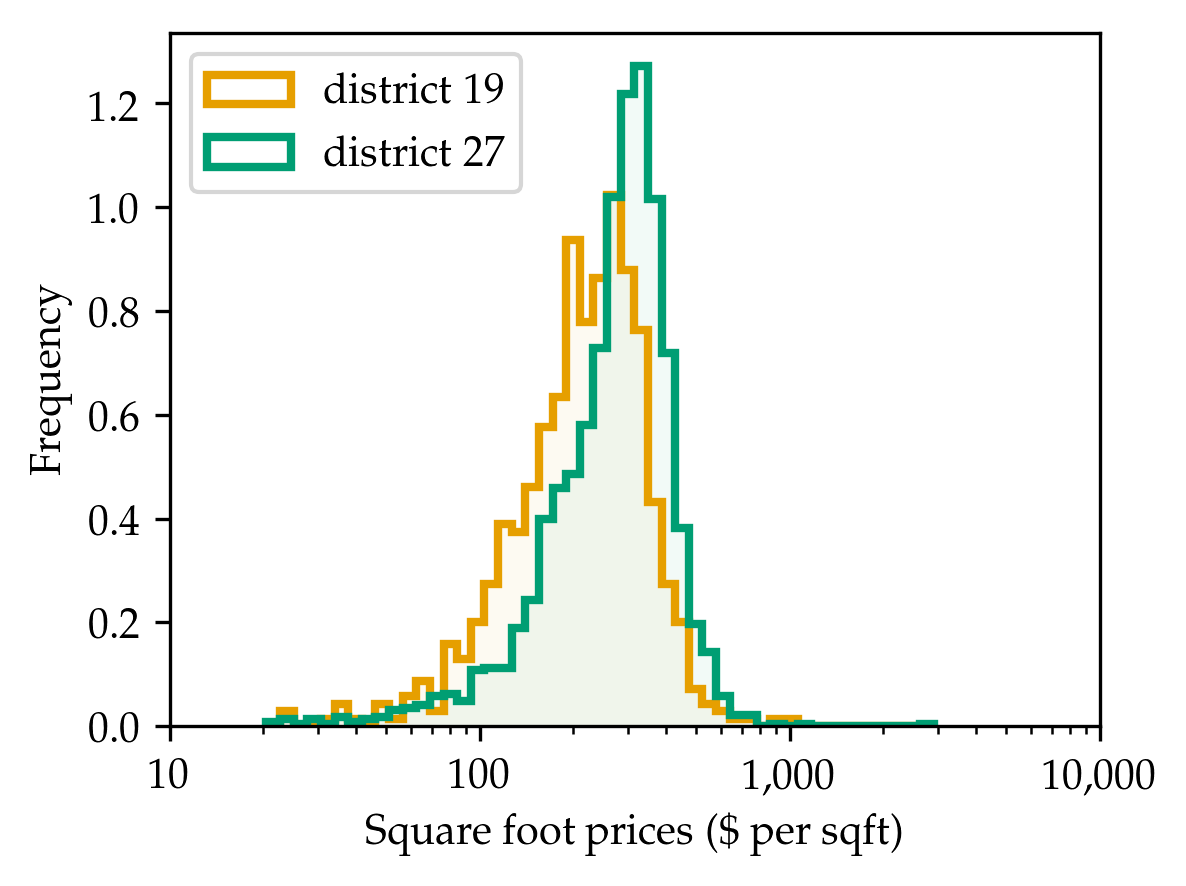
\includegraphics[width=0.4\textwidth]{../NYC/NYC_plots/sales_histogram_19-27.png}
\caption{\label{fig:NYC_histogram}Histogram of log sale prices per square foot in NYC school districts 19 and 27.}
\end{figure}
    


    	We fit the hyperparameters \(\sigma_\beta\), \(\sigmaf\), \(\ell\) and \(\sigman\) by optimizing the marginal log-likelihood of the data within neighboring school districts 18, 19, 23, 24, 25, 26, 27, 28, and 29.
We hold \(\sigmamu\) fixed to 20 to give the district means \(\mu_j\) a fairly uninformative prior.
The fitted hyperparameters were \(\widehat{\sigman}=0.4020\), \(\widehat{\sigmaf}=0.1955\), \(\widehat{\sigma_\beta}=0.1465\), and \(\widehat{\ell}=4482~\text{ft}\).
    


    	\hypertarget{cliff-face-estimator}{%
\subsection{Cliff Face Estimator}\label{cliff-face-estimator}}
    


    	We seek the treatment effect function \(\tau(\border)\) between the two districts.
We could proceed by computing the cliff face estimator with covariates \eqref{eq:cliff_with_covariates}.
But to simplify the analysis as discussed in Section~\ref{sec:covariates}, we can instead obtain the posterior means of the \(\beta_{1j}\) and \(\beta_{2j}\) coefficients (following the procedure outlined in Appendix~\ref{sec:betahat}, but extended to \(J_\district\) rather than just two areas in accordance with~\eqref{eq:nyc_model}), extract the residuals \(\yt{}-\Dmat_\treat{} \hat{\betavec}\) and \(\yc{}-\Dmat_\ctrol{} \hat{\betavec}\), which we then treat as the observed outcomes in a GeoRDD analysis with no non-spatial covariates.
In this example, we find that the posterior variance of \(\betavec\) is low, and therefore the two approaches yield very similar results, but conditioning on the estimate of \(\betavec\) is computationally convenient.
We therefore proceed with this two-step approach.
    


\begin{figure}[tbp]
\centering
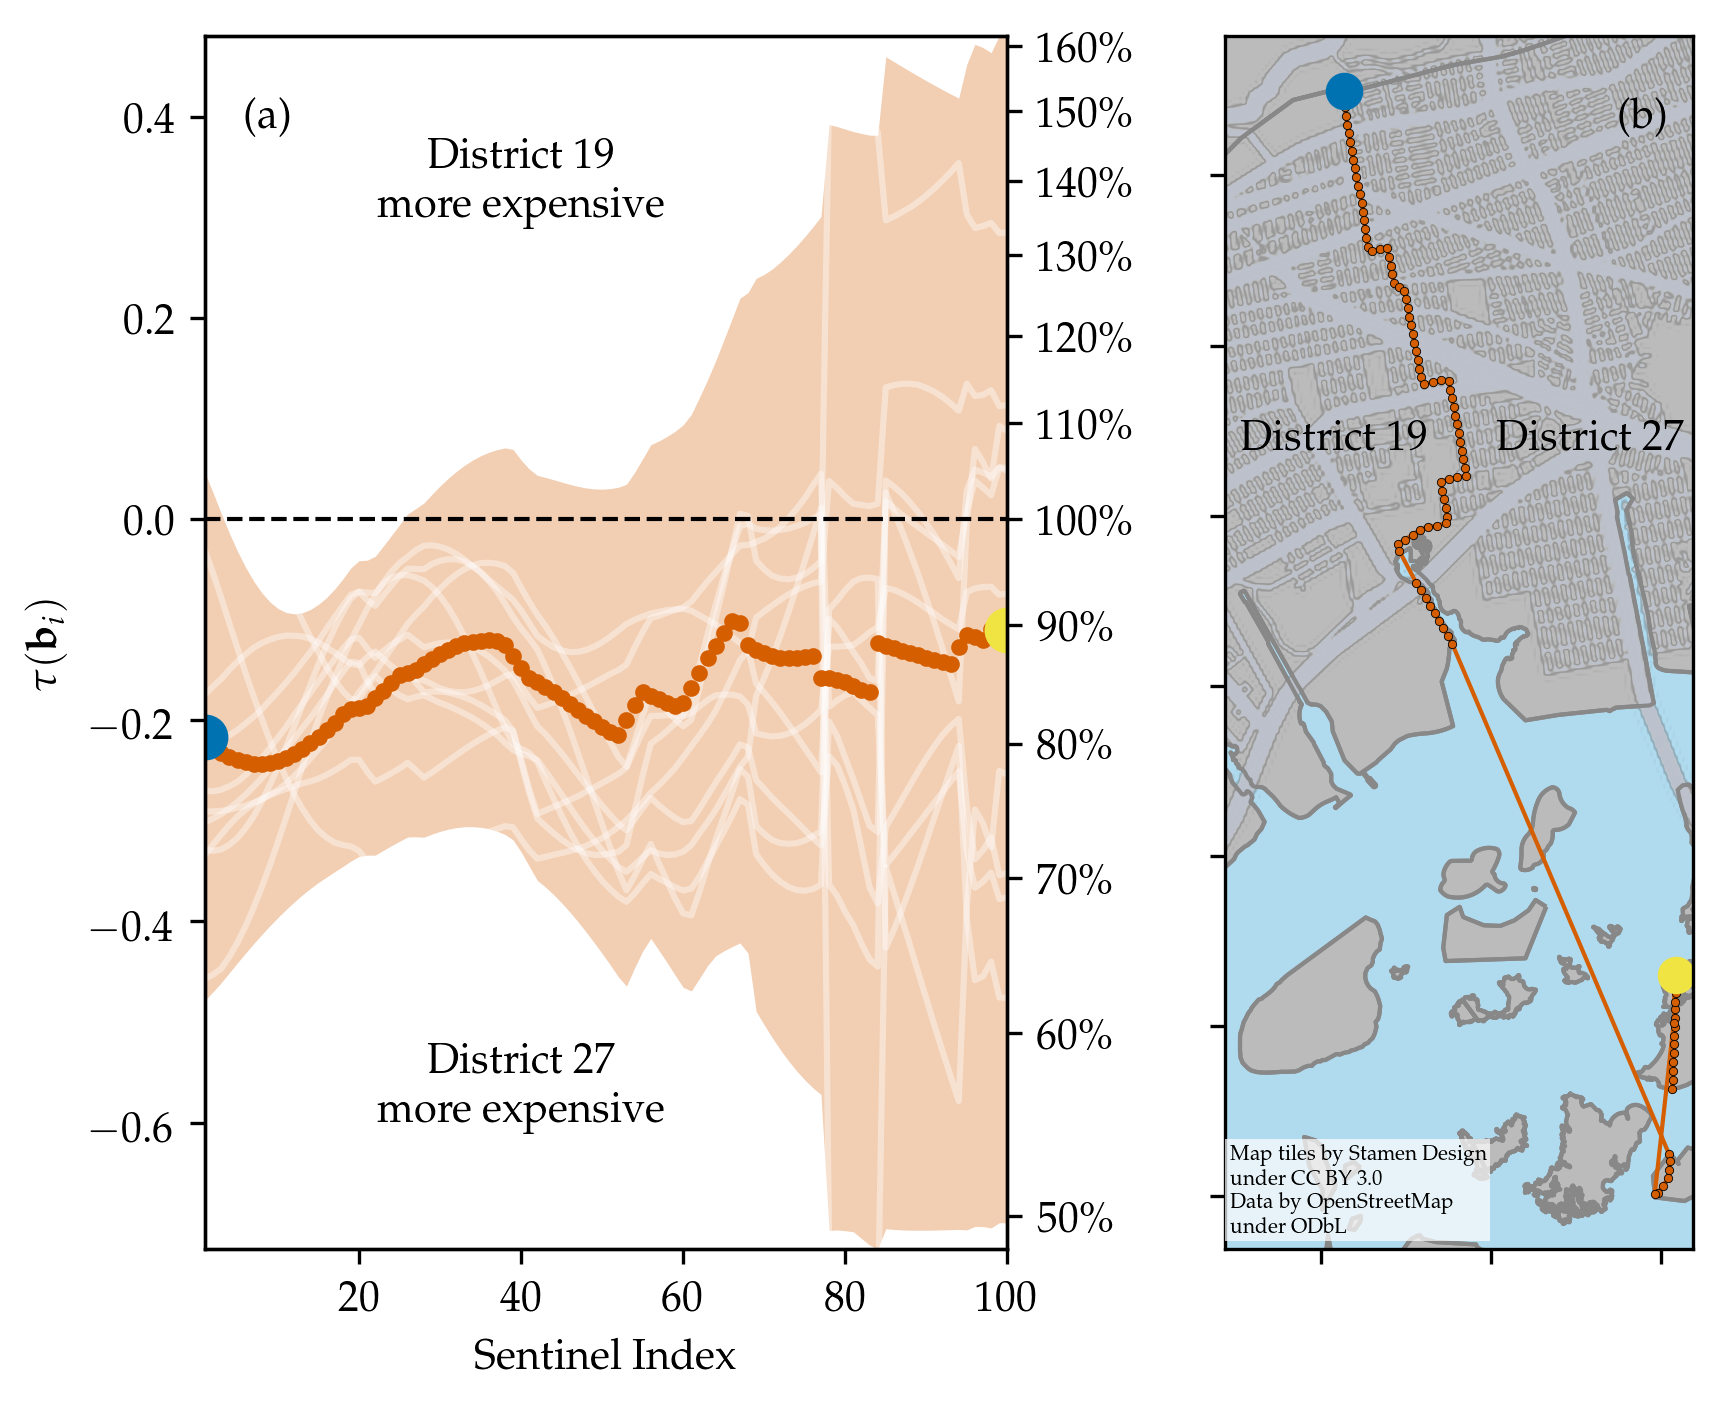
\includegraphics{../NYC/NYC_plots/NYC_cliff_face.png}
\caption{\label{fig:NYC_cliff_face}
(a)
Cliff face estimator for the school district effect on house prices per square foot between district 27 and district 19, with 95\% credible envelope.
The left y-axis is in the scale of log prices per square foot; positive values correspond to houses near the border being more expensive in district 19 than 27.
The right y-axis shows the corresponding ratio of the price of a house near the border in district 19 over its price in district 27.
A few draws from the posterior are shown in lighter color to show the posterior correlations between sentinels.
Note the jumps from sentinels 77 to 78, and 84 to 85, which correspond to the school district border crossing the water from Long Island to islands in Jamaica Bay (Black Wall Island and then Rulers Bar Hassock).
These islands are sparsely populated, and the posterior standard deviation is correspondingly much higher.
(b)
The map of sentinels, evenly spaced along the border between school districts 27 and 19.
The northernmost sentinel---shown as a blue circle in both plots---has index 1, while the last sentinels---shown in yellow---is on Rulers Bar Hassock.}
\end{figure}
    


    	Following the inference procedure outlined in Section \ref{sec:twogp}, we obtain the posterior distribution of the cliff height \(\tau(\border)\) obtained at the sentinel locations.
The cliff face is shown in Figure~\ref{fig:NYC_cliff_face}, and shows that \(\tau(\border)\) is estimated as negative everywhere along the border, which corresponds to higher property prices in district 27.
However, the credible envelope is fairly wide, especially in the southern section of the border, so we cannot visually rule out the null hypothesis that \(\tau(\border)=0\).

The ``cliff face'' can also be visualized directly in Figure~\ref{fig:NYC_3d} as the difference between the two log-price mean surfaces \(g(\svec)\).
The figure also gives a better sense of the spatial variation in prices captured by the model.
    


\begin{figure}[tbp]
\centering
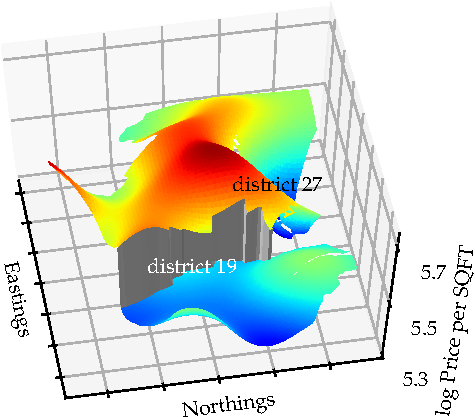
\includegraphics[height=0.35\textheight]{../NYC/NYC_plots/NYC_surface_plot_multi_ev60az170-crop.pdf}
\caption{\label{fig:NYC_3d}NYC surface plot viewed from the West. The grey cliff face connects the fitted price surfaces of districts 19 and 27, and has height given by \eqref{eq:postvar2gp} and shown in Figure~\ref{fig:NYC_cliff_face}.}
\end{figure}
    


    	\hypertarget{average-log-price-increase}{%
\subsection{Average Log-Price Increase}\label{average-log-price-increase}}

The cliff face Figure~\ref{fig:NYC_cliff_face} shows a negative treatment effect everywhere along the border, which can be averaged by the estimators we developed in Section~\ref{sec:ate}.
Our two recommended estimators, based on inverse-variance weighting and finite-population projection, yield ATE estimates of \(-0.19\) and \(-0.18\) respectively, which corresponds to an almost 20\% increase in property prices going from district 19 to district 27.
All ATE estimators from Section~\ref{sec:ate} applied to this setting are shown in Table \ref{table:NYC_ate}.
In this example the different estimators yield similar answers, as the border is fairly straight and short relative to the fitted lengthscale.
    

\begin{table}
\centering
\begin{tabular}{lrrr}
\hline
& \multicolumn{3}{c}{Posterior} \\
    Estimand & Mean & Standard Dev. & Tail Prob. \\
    \hline
$\unifavg$ & -0.17 & 0.09 & 2.93\% \\
$\taurho$  & -0.19 & 0.06 & 0.04\% \\
$\invvar$  & -0.19 & 0.06 & 0.03\% \\
$\tauproj$ & -0.18 & 0.08 & 1.31\% \\
$\taugeo$  & -0.16 & 0.09 & 3.99\% \\
$\taupop$  & -0.18 & 0.06 & 0.08\% \\
\hline
\end{tabular}
\label{table:NYC_ate}
\caption{Average difference in log price per square foot between school districts 19 and 27. For each ATE estimand, we show the mean and standard deviation of its posterior distribution, and the tail probability $\Pr(\tau > 0 \mid Y, \hat{\beta}, \hyperparam)$ of the average treatment being greater than zero. Negative ATEs correspond to district 27 being more expensive.}
\end{table}
    	\hypertarget{significant-difference-in-price}{%
\subsection{Significant Difference in Price?}\label{significant-difference-in-price}}

The inverse-variance weighted mean treatment effect estimated suggests a significant treatment effect.
But the posterior tail probability cannot be interpreted as a \(p\)-value.
For this, we turn to the three tests developed in Section~\ref{sec:hypothesis_testing}.
In applied settings, running multiple tests should be done with care,
but as we are proposing this new methodology,
we apply all three tests in order to gain insight into their differences.
Their results are found in Table~\ref{table:NYC_tests}.
    

\begin{table}[tbp]
\centering
\label{table:NYC_tests}
\begin{tabular}{ll}
\hline
Test                   & $p$-value \\
\hline
$\chi^2$ bootstrap     & 0.012     \\
mLL bootstrap          & 0.002     \\
$\invvar$ uncalibrated & 0.0007    \\
$\invvar$ calibrated   & 0.002 \\
\hline
\end{tabular}
\caption{Results of hypothesis tests for New York school district house prices.}
\end{table}
    	The three tests reject the null hypothesis that \(\tau\del{\border}=0\) along the border between districts 19 and 27.
This will not always be the case, as the calibrated inverse-variance test has higher power than the other two tests.
The \(\chi^2\) test had the lowest power in the simulated example of Section~\ref{sec:powersim}, and here also returns the highest \(p\)-value.
    


    	To assess the validity of the three tests, we apply the placebo tests devised in Section~\ref{sec:placebo}.
Within each district, we split the data in half by a line at angles \(1\degree\), \(3\degree\), \(5\degree\), \(6\degree\), \(\dotsc\), \(179\degree\).
Because these lines were drawn arbitrarily, we don't expect a discontinuous treatment effect between the two halves, and so we hope to see a uniform distribution of placebo \(p\)-values.
However, these tests will be highly correlated,
and so the low effective sample size could lead to some apparent departures from uniformity.
There is in fact visible autocorrelation in the graphs of placebo \(p\)-values as a function of angle.
    
\begin{figure}[tbp]
\centering
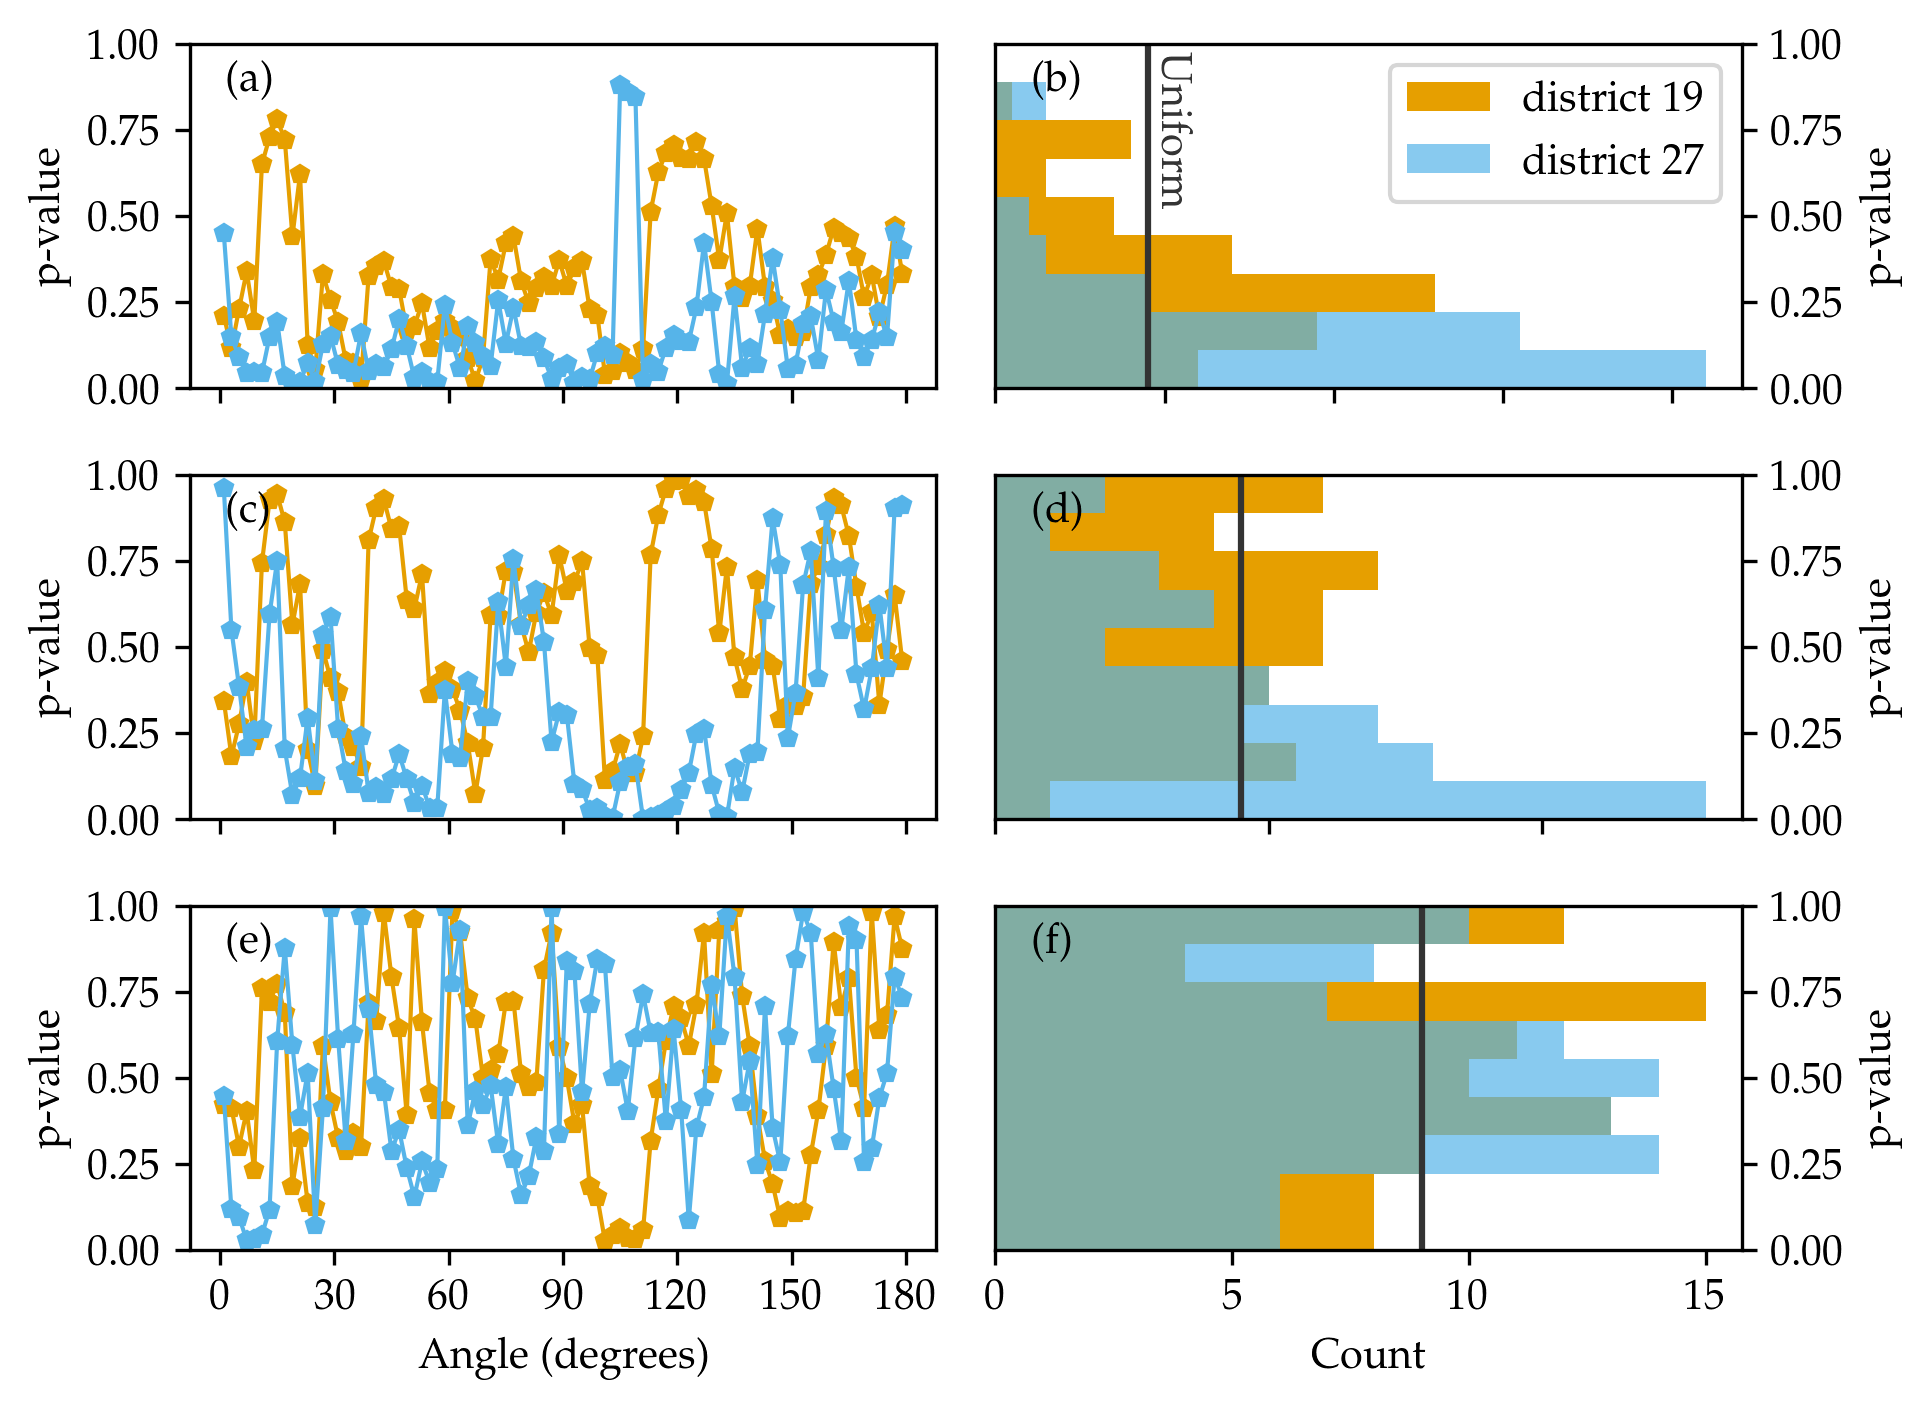
\includegraphics[width=\textwidth,height=0.4\textheight,keepaspectratio]{../NYC/NYC_plots/NYC_placebos.png}
\caption{\label{fig:nyc_placebos} Placebo tests for significance tests applied to NYC school district house prices, applied within districts 19 and 27. The three rows respectively show results for the marginal log-likelihood bootstrap test, chi-squared bootrap test, and calibrated inverse-variance test. The first column shows the placebo p-value as a function of the border angle; the second column shows histograms of the placebo p-values, with the black vertical line indicating the uniform distribution.}
\end{figure}

    	The mLL placebo \(p\)-values show a pronounced bias towards low values.
This seems to confirm our concern that the marginal log-likelihood may be sensitive to features of the data other than the discontinuity at the border.
In particular, model misspecification, which is a concern in spatial models, makes the interpretation of the mLL test unreliable.
Based on this vulnerability, and its manifestation in this application, we do not recommend relying on the likelihood-ratio test.

The \(\chi^2\) test shows more robustness, with Figure~\ref{fig:nyc_placebos}(d) showing some negative bias in district 27, and some positive bias in district 19, which could simply be due to the low effective sample size.
We therefore believe that the \(\chi^2\) test will continue to be reliable under misspecification.
It is only due to its low power that we hesitate to recommend its use in applications where the treatment effect is expected to be fairly homogenous.

Lastly, the calibrated inverse-variance placebo \(p\)-values display no obvious bias, with Figure~\ref{fig:nyc_placebos}(f) close to uniformly distributed, and Figure~\ref{fig:nyc_placebos}(e) showing a lower auto-correlation than the mLL and \(\chi^2\) tests.
The high power and robustness of the inverse-variance test make a strong case for its use in most applications.
    


    	\hypertarget{pairs-of-school-districts}{%
\section{Pairs of School Districts}\label{pairs-of-school-districts}}
    


    	The GeoRDD analysis can be repeated for each pair of adjacent districts.
Figure~\ref{fig:NYC_pairwise} and Table~\ref{table:NYC_pairwise} give an overview of the results by showing the posterior mean and standard deviation of the inverse variance ATE estimated at each border.
Significant effects are found between many districts, but interpreting the results requires some caution.
We have already mentioned the issue of compound treatments for borders between school districts that overlap with the border between boroughs.
School districts 19, 32, and 14 are in Brooklyn, while districts 30, 24, and 27 are in Queens.
    

\begin{figure}[tbp]
\centering
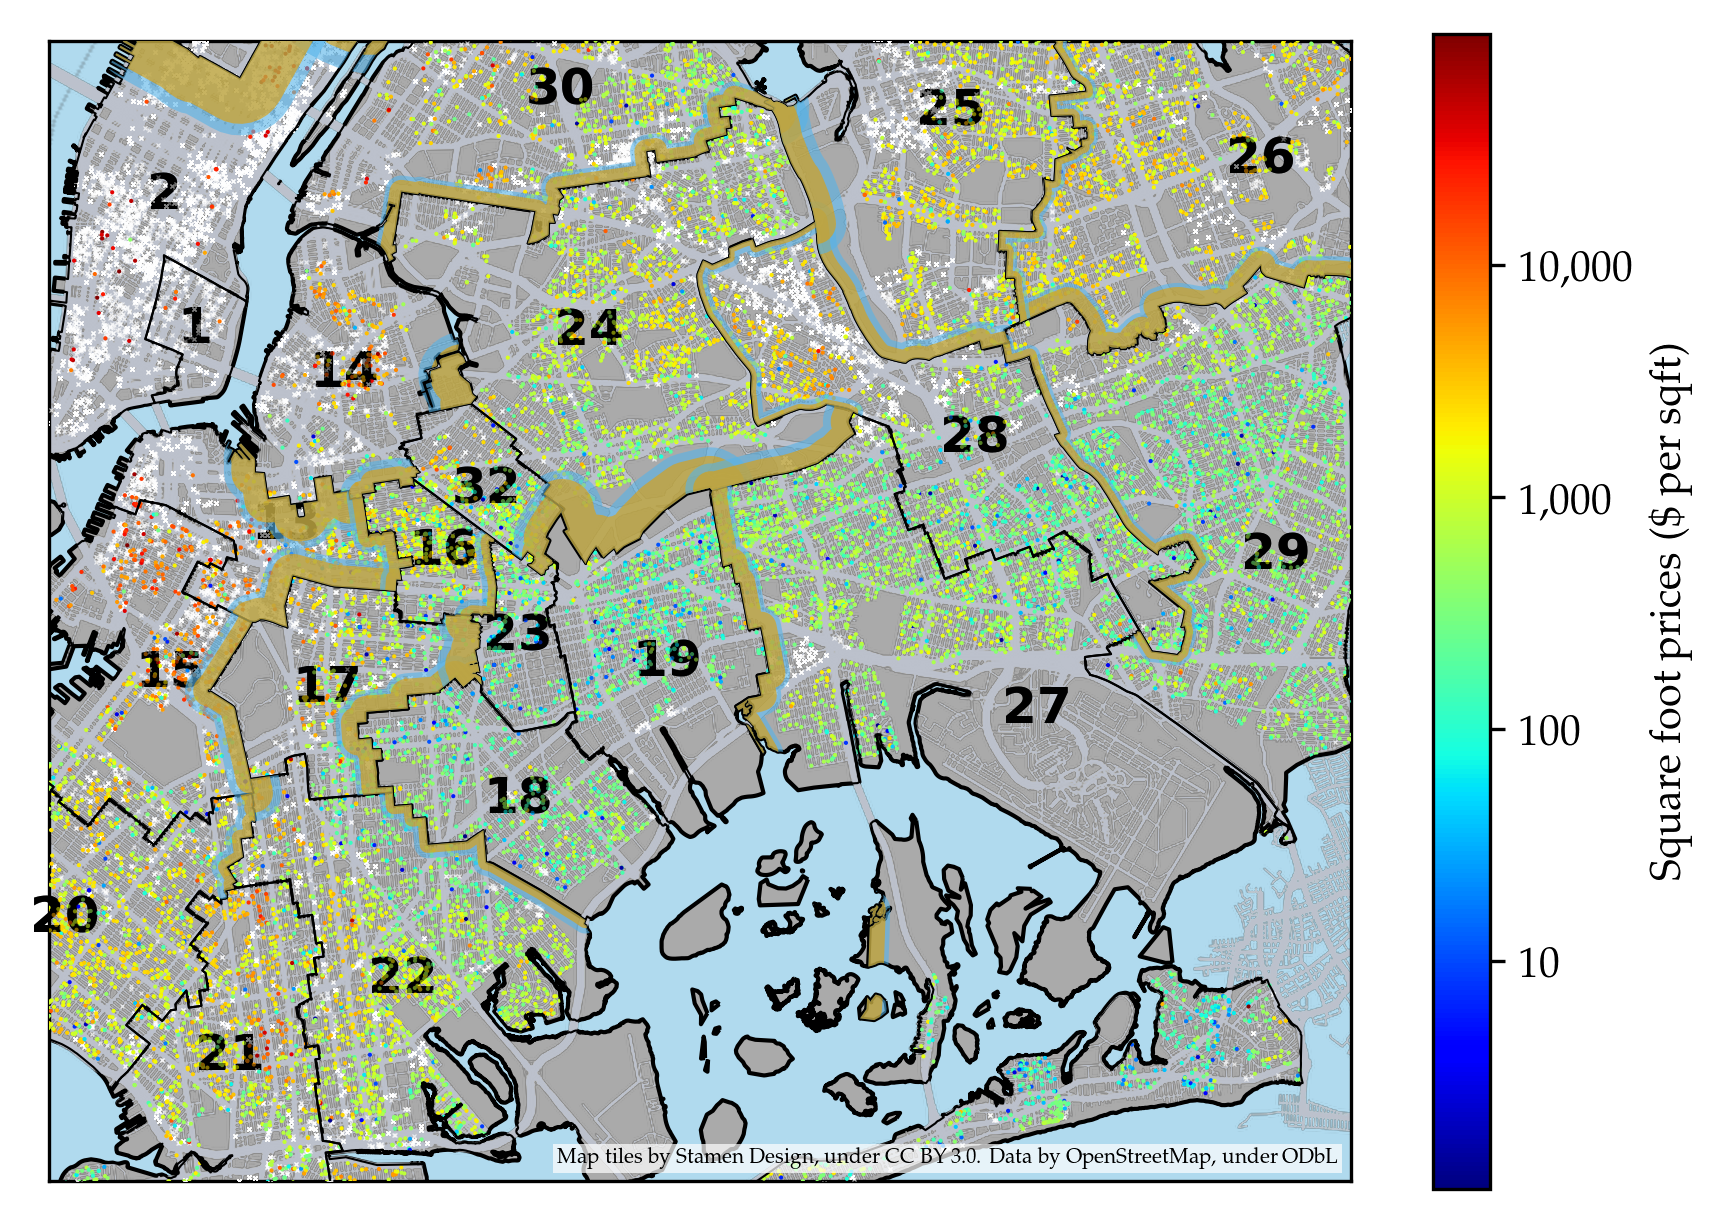
\includegraphics[width=\textwidth,height=0.7\textheight,keepaspectratio]{../NYC/NYC_plots/pairwise_mean_se.png}
\caption{\label{fig:NYC_pairwise}
Pairwise estimates of the inverse variance ATE between adjacent districts.
The thickness of the orange buffer adjacent to borders is proportional to the posterior mean of the inverse variance ATE, and the blue buffer beyond it is proportional to the posterior standard deviation of the ATE.
The buffers are drawn on the side of the border that is estimated to have higher house prices.}
\end{figure}

    	Some school districts are separated by parks (or other non-residential zones), for example districts 15 \& 17 or 19 \& 24, so that house sales do not extend all the way to the border on one or both sides.
A significant treatment effect between these pairs cannot be interpreted as the detection of a discontinuity in prices at the border, let alone any kind of causal interpretation, but rather it means that the difference in prices between the two sides of the park exceeds the typical spatial variation of house prices expected over the same distance.
This is not unsurprising, and one may speculate that physical barriers like parks, rivers, railways and major roads can separate neighborhoods with distinct character, demographics and thus house prices.
This in turn challenges the stationarity assumption of the spatial model \eqref{eq:spec2gp}.
The higher distance between data and the border also stretches the spatial model's ability to extrapolate, which makes it more vulnerable to model misspecification.
And it violates the assumptions
    



    	Other pairs of district, like 13 \& 14, 13 \& 17, and 25 \& 28 have clusters of missing data (condo sales with unknown square footage) near the border that cast doubt on the interpretation of the estimated effect.
Nonetheless, significant effects are also found between pairs of school districts without issues due to compound treatments, physical barriers, or missing data.
House prices increase going across the border from districts 16 to 13, 18 to 17, 24 to 30, 23 to 17, 25 to 26, 28 to 29, and 29 to 26.
Overall, it seems that school district borders in Brooklyn and Queens can correspond to measurable jumps in house prices per square foot.
The estimated size of this effect varies: zero or negligible in some cases, such as between districts 15, 20, 21, and 22; and quite pronounced in others, such as a 20\% price increase from 29 to 26, or 22\% from 18 to 17.
    


    	\hypertarget{conclusion}{%
\section{Conclusion}\label{conclusion}}
    


    	Geographic regression discontinuity designs (GeoRDDs) arise when a treatment is assigned to one region, but not to another adjacent region.
For outcomes that vary spatially, a direct comparison of mean outcomes between \(\yt\) and \(\yc\), such as a \(t\)-test, is an invalid estimator of the treatment effect, as it is confounded by the spatial covariates.
However, under smoothness assumptions, units adjacent to the border are comparable, and form a natural experiment.
The same idea underpins causal interpretations of one-dimensional regression discontinuity designs (1D RDDs), where a single ``forcing'' variable controls the treatment assignment instead of a border separating two geographical regions.
We use this similarity to motivate a general framework for the analysis of GeoRDDs.
One-dimensional methods can be abstracted to three steps: (1) fit a smooth function on either side of the threshold; (2) extrapolate the functions to the threshold; and (3) take the difference of the two extrapolations to estimate the treatment effect at the threshold.
For GeoRDDs we propose to (1) fit a smooth surface on either side of the border; (2) extrapolate the surfaces to the border; and (3) take the difference of the two extrapolations to estimate the treatment effect along the border.

Previous research has focused on extending methods developed for 1D RDDs to GeoRDDs.
In applied settings, some have used the signed distance from the border as the forcing variable in a 1D RDD, but the resulting estimator is still spatially confounded.
In this paper, our aim was to recognize the importance of the geographical aspect of the problem, and therefore draw from the spatial statistics literature, which brings a rich set of tools designed specifically to model and exploit spatial correlations to obtain more powerful inference.
We therefore used Gaussian process regression, known as kriging in the spatial statistics literature, to fit the smooth surfaces to the outcomes in step (1) of our general framework.
Our approach yields a multivariate normal posterior distribution of the treatment effect for a collection of ``sentinel'' locations along the border.
    


    	Defining an ``average treatment effect'' estimand turns out to have surprising pitfalls.
Simply integrating the treatment effect uniformly along the border yields an estimand that is inefficient and undesirably sensitive to the topology of the border.
More sophisticated estimands, summarized in Table~\ref{table:estimator_properties}, are robust to this effect, and use the information available in the data more efficiently.

There are multiple valid approaches to hypothesis testing against the null hypothesis of zero treatment effect along the border.
We recommend the use of the calibrated inverse-variance test, derived from the posterior distribution of the inverse-variance ATE estimator.
It has generally high statistical power and behaved well in placebo tests in the NYC application.
    


    	We applied our method to a publicly available dataset of one year of New York City property sales, to examine whether school district cause difference in property prices.
Focusing on the border between school districts 19 and 27, we estimated a roughly 20\% average increase (inverse variance ATE) in house prices per square foot when crossing the border from district 19 to district 27.
However, the border between these two districts is also the border between the NYC boroughs of Brooklyn and Queens, so we cannot attribute this difference to the causal effect of the school districts.
Other limitations apply to many pairs of districts.
Parks, commercial zones, railways, and major roads can separate neighborhoods, keep data away from the borders, break the stationarity assumption of the spatial model, and increase the amount of extrapolation performed by the model, which casts doubt on the legitimacy of the estimated treatment effects.
Missing data from condo sales which do not report square footage can also distort estimated effects.
Some pairs of adjacent school district remain where a large effect was found, such as a the 22\% increase in house prices per square footage when crossing the border from district 18 to 17.
Overall, it seems that school district borders in Brooklyn and Queens are often accompanied by a discontinuity in house prices, but the causal attribution of this difference to the reputation of the school districts is often questionable due to the aforementioned geographical and political complications.
    


    	The main limitation of our approach to GeoRDDs is the reliance on modeling assumptions.
We modeled the response surfaces as two independent Gaussian processes, with iid normal noise for each observation.
As is common in spatial statistics, we use Gaussian processes as non-parametric smoothing devices used to capture spatial correlations, but do not think of them as truthful approximations to the data generating mechanism.
We believe care must be taken not to lean heavily on this modeling assumption.
In particular, we recommend that hypothesis tests always be accompanied by placebo tests:
by applying the same procedure on data where no treatment was applied, we can verify that the test behaves appropriately under the null hypothesis despite any potential model misspecification.
We also assumed a stationary covariance structure, with hyperparameters equal in the treatment and control regions, and in particular we chose the squared exponential kernel.
This kernel makes smoothness assumptions that are often considered unrealistic in spatial settings, and so the Matérn covariance family is often recommended as a more robust alternative.
The assumption of equal covariance parameters in the two areas can also be relaxed, by separately tuning the parameters within each area.

Because of the need to extrapolate the fitted processes a short distance to the border, our GeoRDD method may be vulnerable to the limitations of Gaussian processes when extrapolating.
The distinction between interpolation and extrapolation of spatial models is explored in some depth in \cite{stein2012interpolation}.
We expect that methodological advances that improve the extrapolating behavior of Gaussian processes would also improve the robustness of our method.
For example, \cite{wilson2013gaussian} develop spectral mixture (SM) covariance kernels with good extrapolating behavior, which could be applied beneficially to GeoRDDs.
However, SM kernels are motivated by time series with some periodic or oscillatory behavior, which is more unusual in spatial applications, and may therefore not be as well-suited for use with GeoRDDs.
    


    	The use of Gaussian process regression to analyse GeoRDDs gives flexibility and extensibility to the method.
This presents many opportunities for future research, inspired by the past and future development of methods in spatial statistics and machine learning that are based on Gaussian processes.
In spatial statistics, kriging has been used as the foundation for a plethora of spatial models, which may be adapted for the purposes of analyzing GeoRDDs.
\cite{banerjee2014hierarchical} provides a good introduction to the richness of the spatial statistics field.
For example, if the outcomes are binary, proportions, or counts, then binomial or Poisson likelihoods could be substituted for the iid normal likelihood used in this paper.
Besides ATE and hypothesis testing, another potential question is whether the treatment effects are homogenous or heterogeneous.
Hypothesis tests of homogeneity would be an interesting possible extension of our framework.

The framework and techniques of this paper could also be extended to spatio-temporal settings.
If the treatment is only applied to the treatment region after a time \(t*\), one could envision a three-dimensional RDD consisting of the geographical border in the spatial dimensions, and a straight line through \(t*\) in the temporal dimension.
The only necessary modification to our approach is that the Gaussian process model would need to be augmented with a temporal component, for example with an anisotropic squared exponential covariance function.
Longitudinal studies could also be handled by such an approach, with the addition of random intercepts for each unit.
We leave spatio-temporal RDDs using Gaussian process models to future research.
    


    	\appendix
    


    	\hypertarget{spatial-confounding-of-1d-rdd-applied-to-geordd}{%
\section{Spatial Confounding of 1D RDD Applied to GeoRDD}\label{spatial-confounding-of-1d-rdd-applied-to-geordd}}
    


    	\label{sec:confounding}
    


    	Analysing GeoRDDs by using the signed distance from the border as a forcing variable in a 1D~RDD can lead to spatial confounding.
We demonstrate this with a simple artificial example, depicted in Figure~\ref{fig:confounding}.
    


\begin{figure}[tbp]
\centering
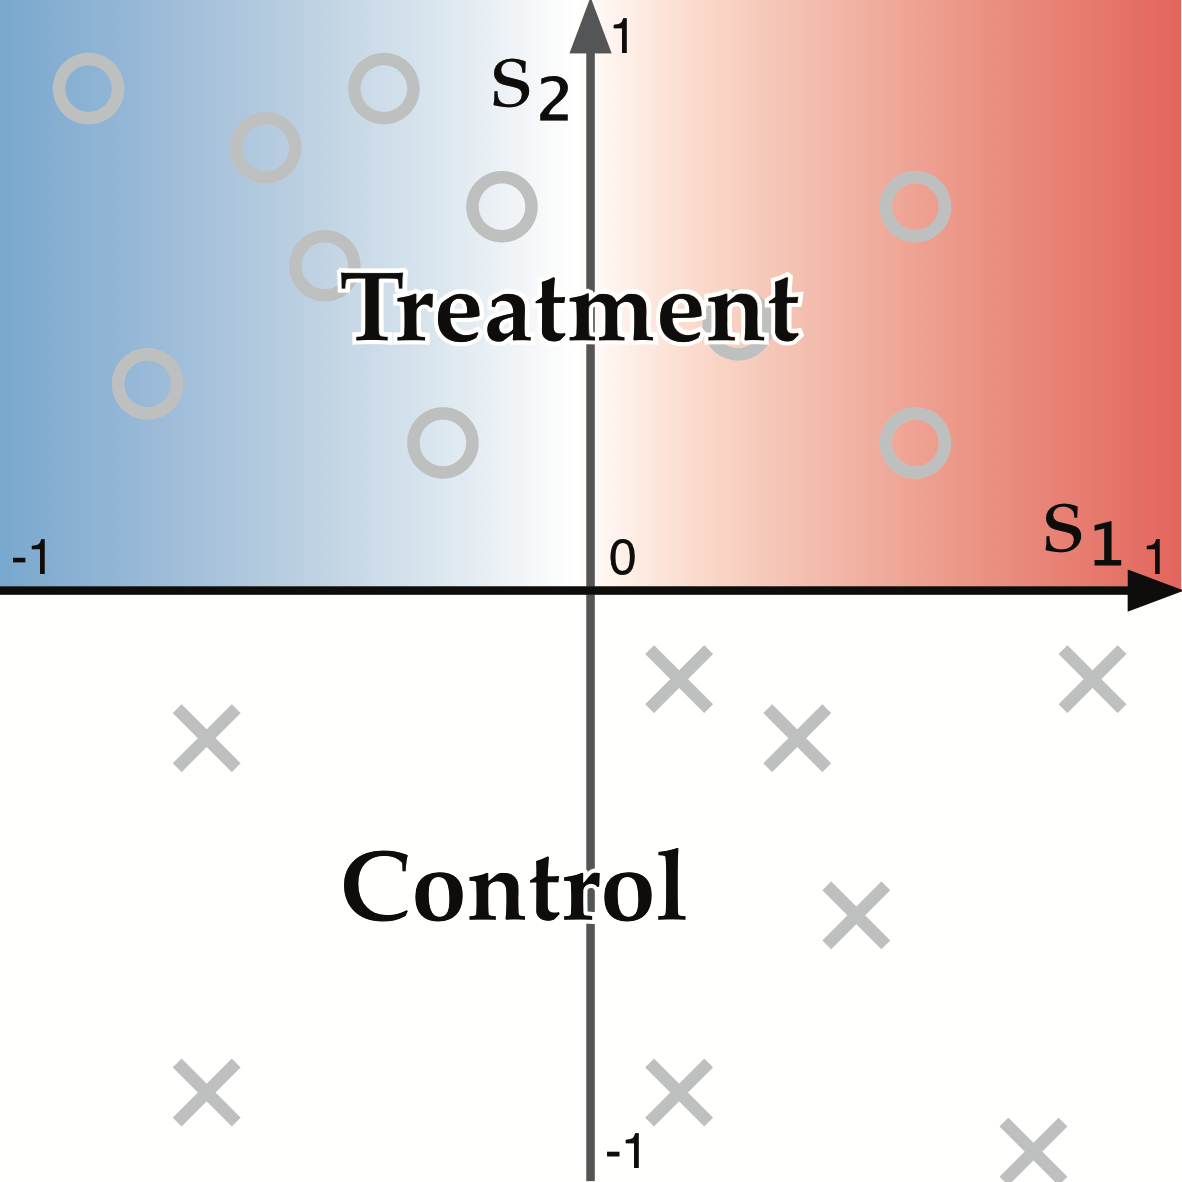
\includegraphics[height=0.35\textheight]{figures/confounding/confounding.png}
\caption{A theoretical example illustrating the susceptibility of the projected 1D~RDD method to spatial confounding. The locations of treatment and control units are shown with circles and crosses respectively, separated by a border at \(s_2 = 0\). Units are denser in the upper left and lower right quadrants. The treatment effect, depicted as a gradient from blue to red, increases linearly with \(s_1\). \label{fig:confounding}}
\end{figure}
    


    	Suppose we have units in a 2D square, with spatial coordinates \(\svec_1 \in [-1,1]\), and \(\svec_2 \in [-1,1]\), and with a horizontal border at \(s_2=0\) separating a treatment region from a control region.
Let us assume the null hypothesis, with outcomes driven only by \(\svec_1\) (parallel to the border), given by \(Y_{i} = \alpha \svec_{1i} + \epsilon_i\),
where \(\epsilon_i\) is an iid noise term \(\epsilon_i \sim \normal\del{0, \sigman^2}\).
Lastly, let us consider the situation where the density \(\rho(\svec)\) of units is different in each quadrant of the square:
\begin{equation}
\begin{aligned}
    \rho(\svec) = 2\rho_0 & \text{, where }\svec_1 < 0,~\svec_2 > 0 & \text{ (top left)} \\
    \rho(\svec) = \rho_0 & \text{, where }\svec_1 > 0,~\svec_2 > 0 & \text{ (top right)} \\
    \rho(\svec) = 2\rho_0 & \text{, where }\svec_1 > 0,~\svec_2 < 0 & \text{ (bottom right)}  \\
    \rho(\svec) = \rho_0 & \text{, where }\svec_1 < 0,~\svec_2 < 0 & \text{ (bottom left)}
\end{aligned}
\end{equation}
The projection RDD then considers a 1D RDD along \(s_2\).
The usual RDD estimand \eqref{eq:rdd_univ_estimand} can be obtained analytically, and equals \(\tau=\frac{-\alpha}{3}\), despite assuming the null hypothesis.
This is because \(s_1\) acts as a hidden confounder, whose distribution changes discontinuously at the border, which leads to bias and inconsistency in the projected 1D~RDD estimate.
In geographical settings, a discontinuous change in the density of units at the border is not unusual: for example a border could run alongside a park, or a small body of water, therefore with zero population density on one side of the border.
A visual inspection of Figure \ref{fig:sales_map} showing the locations of units in a New York City property sales dataset reveals many examples of this.
    


    	\hypertarget{covariances-for-gaussian-process-model}{%
\section{Covariances for Gaussian Process Model}\label{covariances-for-gaussian-process-model}}
    

\label{sec:covariances}
    	All covariances below are conditional on the hyperparameters \(\hyperparam = \del{\ell,\sigmaf, \sigman, \sigmamu}\), omitted for concision.
    


    	\begin{equation}
\begin{split}
    m_\treat, m_\ctrol   &\sim \normal\del{0,\sigmamu^2} \\
    \cov(Y_{i\treat},m_\treat)  &= \sigmamu^2 \\
    \cov(Y_{i\ctrol},m_\ctrol)  &= \sigmamu^2 \\
    \cov(Y_{i\treat},m_\ctrol)  &= \cov(Y_{i\ctrol},m_\treat)  = 0 \\
    \cov\del{Y_{i\treat}, f_{\treat}(\svec')} &= k(\svec_i,\svec') \\
    \cov\del{Y_{i\ctrol}, f_{\ctrol}(\svec')} &= k(\svec_i,\svec') \\
    \cov\del{Y_{i\treat}, f_{\ctrol}(\svec')} &= \cov\del{Y_{i\ctrol}, f_{\treat}(\svec')} = 0 \\
    \cov(Y_{i\treat},Y_{j\treat}) &= \cov(Y_{i\ctrol},Y_{j\ctrol}) = \sigmamu^2 + k(\svec_i,\svec_j) + \delta_{ij}\sigman^2 \\
    \cov(Y_{i\treat},Y_{j\ctrol}) &= 0
\end{split}
\eqlabel{eq:covariances}
\end{equation}
    


    	We further define some shorthand notation, found in the table below.

\begin{center}
\begin{tabular}{lll}
\hline
Symbol & Size                       & $ij^{\mathrm{th}}$ entry                                                      \\ \hline
$\KBB$ & $\numsent \times \numsent$ & $\sigma_m^2 + k\del{\sentinel_i,\sentinel_j}$                                 \\ 
$\KBT$ & $\numsent \times n_\treat$ & $\sigma_m^2 + k\del{\sentinel_i,\svec_{j\treat}}$                             \\ 
$\KBC$ & $\numsent \times n_\ctrol$ & $\sigma_m^2 + k\del{\sentinel_i,\svec_{j\ctrol}}$                             \\
$\KTT$ & $n_\treat \times n_\treat$ & $\sigma_m^2 + k\del{\svec_{i\ctrol},\svec_{j\ctrol}}$                         \\
$\KCC$ & $n_\ctrol \times n_\ctrol$ & $\sigma_m^2 + k\del{\svec_{i\treat},\svec_{j\treat}}$                         \\ 
$\STT$ & $n_\treat \times n_\treat$ & $\sigma_m^2 + k\del{\svec_{i\treat},\svec_{j\treat}} + \delta_{ij} \sigman^2$ \\ 
$\SCC$ & $n_\ctrol \times n_\ctrol$ & $\sigma_m^2 + k\del{\svec_{i\ctrol},\svec_{j\ctrol}} + \delta_{ij} \sigman^2$ \\
\hline
\end{tabular}
\end{center}

    	\hypertarget{posterior-mean-of-betavec}{%
\section{\texorpdfstring{Posterior Mean of \(\betavec\)}{Posterior Mean of \textbackslash{}betavec}}\label{posterior-mean-of-betavec}}

\label{sec:betahat}

We derive the posterior mean of the linear regression coefficients vector \(\betavec\) for the model specified in \eqref{eq:covariates_model}.
    


    	\begin{equation}
\begin{aligned}
    \Yvec &= \begin{pmatrix}
            \yt \\
            \yc
        \end{pmatrix}
        \\
    \SigmaMat_{Y \mid \beta} &= \cov\del{\Yvec \mid \betavec }
        = \begin{bmatrix}
            \STT & 0 \\
            0 & \SCC
          \end{bmatrix}
        & \text{conditional variance of $Y$} \\
    \cov\del{\betavec} &= \sigmabeta^2 \eye_p
        & \text{prior variance of $\betavec$} \\
    \SigmaMat_Y &= \cov\del{\Yvec} 
            = \SigmaMat_{\Yvec \mid \betavec} 
              + \sigmabeta^2 \Dmat \Dmat\trans
        & \text{prior variance of $\Yvec$} \\
    \hat\betavec &= \sigmabeta^2 \Dmat\trans\SigmaMat_{Y}^{-1} \Yvec
        & \text{posterior mean of $\beta$}
\end{aligned}
\end{equation}
    


    	The treatment and control residuals can then be obtained respectively as \(\residvec_\treat = \yt - \Dmat_\treat \hat\betavec\) and \(\residvec_\ctrol = \yc - \Dmat_\ctrol \hat\betavec\).
Conditionally on \(\hat\betavec\), the residuals \(\residvec_\treat\) and \(\residvec_\ctrol\) then have independent multivariate normal distributions with the same mean and covariance as \(\yt\) and \(\yc\) respectively.
    


    	\hypertarget{calibration-of-inverse-variance-test}{%
\section{Calibration of Inverse-variance Test}\label{calibration-of-inverse-variance-test}}
    


    	\label{sec:calibration}
    


    	We seek to obtain a valid hypothesis test against the null hypothesis of zero treatment effect everywhere along the border by using the inverse-variance weighted ATE estimate obtained in Section~\ref{sec:invvar} as a test statistic.
    


    	Under the parametric null hypothesis \(\modnull\), \(\yt{}\) and \(\yc{}\) are drawn from a single Gaussian process, with no discontinuity at the border.
Their joint covariance is
\begin{equation}
    \cov \del{\begin{pmatrix}\yt{} \\ \yc{}\end{pmatrix} \mid \modnull } 
    = \begin{bmatrix}
        \STT & \KTC \\
        \KTC \trans & \SCC
    \end{bmatrix}\,,
\end{equation}
where \(\KTC\) is the \(n_\treat \times n_\ctrol\) matrix with \(ij^{\mathrm{th}}\) entry equal to \(k\del{\svec_{i\treat},\svec_{j\ctrol}}\).
The predicted mean outcomes \eqref{eq:postvar2gp_t_or_c} at the sentinels \(\mu_{\sentinels \mid T}\) and \(\mu_{\sentinels \mid T}\) are obtained by left-multiplying \(\yt{}\) and \(\yc{}\) by matrices \(\AT{}\) and \(\AC{}\) (respectively) that are deterministic functions of the unit locations and the hyperparameters:
\begin{equation}
\begin{split}
    \AT &= \KBT \STT^{-1} \,\text{, and} \\
    \AC &= \KBC \SCC^{-1}\,.
\end{split}
\end{equation}
    


    	Under \(\modnull\), the joint distribution of \(\mu_{\sentinels \mid T}\) and \(\mu_{\sentinels \mid T}\) is consequently also multivariate normal with mean zero and covariance given by:
\begin{equation}
    \cov \del{\begin{pmatrix}\AT{} \yt{} \\ \AC{} \yc{} \end{pmatrix} \mid \modnull } = \begin{bmatrix}
                        \AT{} \STT \AT{}\trans & \AT{} \KTC \AC{}\trans \\
                        \del{\AT{} \KTC \AC{} \trans}\trans & \AC{} \SCC \AC{}\trans
                    \end{bmatrix}\,.
\end{equation}
Continuing in this fashion, the cliff-face estimate \(\mu_{\sentinels \mid Y}\) \eqref{eq:postvar2gp} is yet another zero-mean multivariate normal with covariance given by:
    	\begin{equation}
\begin{split}
    \cov \del{\mu_{\sentinels \mid Y} \mid \modnull} &= \cov\del{ \AT{} \yt{} - \AC{} \yc{} } \\
        &= \AT{} \STT \AT{}\trans + \AC{} \SCC \AC{}\trans - \AT{} \KTC \AC{}\trans -  \del{\AT{}\KTC \AC{}\trans}\trans \,.
\end{split}
\end{equation}
    


    	Weighted mean ATE estimators of the form defined in \eqref{eq:weighted_estimator} are linear transformations of \(\mu_{\sentinels \mid Y}\) and so under \(\modnull\), they are normally distributed with mean zero.
For a weight function \(\weightb(\sentinel)\), its variance is given by
\begin{equation}
\begin{aligned}
    \var\del{\mu_{\tauw \mid Y} \mid \modnull} &= \cov\del{ \frac{\weightb(\sentinels)\trans \mu_{\sentinels \mid Y}}{\ones_{\numsent}\trans \weightb(\sentinels)}} \\
    &= \frac{\weightb(\sentinels) \trans \cov \del{\mu_{\sentinels \mid Y}} \weightb(\sentinels)}{\del{\ones_{\numsent}\trans \weightb(\sentinels)}^2}
    \,.
\end{aligned}
\end{equation}
    

    	The \(p\)-value follows from treating the ATE estimate as a test statistic.
Under the null hypothesis, the probability of \(\mu_{\tauw \mid Y}\) exceeding in magnitude its observed value \(\mu_{\tauw \mid Y}^{obs}\) is:
\begin{equation}
    \Pr\del{ \abs{\mu_{\tauw \mid Y}} > \abs{\mu_{\tauw \mid Y}^{obs}} \mid \modnull} = 2 \Phi\del{ -\frac{\abs{\mu_{\tauw \mid Y}^{obs}}}{\sqrt{\var\del{\mu_{\tauw \mid Y} \mid \modnull}}} }\,.
\end{equation}
The calibrated inverse-variance introduced in Section~\ref{eq:calib_test} test is the special case of this procedure where the weights are chosen to be \(\weightb(\sentinels) = \Sigma^{-1}_{\sentinels \mid Y} \ones_{\numsent}\).
    

\newgeometry{margin=2cm} % modify this if you need even more space
\begin{landscape}

\hypertarget{tables}{%
\section{Tables}\label{tables}}
\label{sec:tables}

\begin{table}[!h]
\begin{tabular}{r|rrrrrrrrrrrr}
\hline
	$n_{\mathrm{wiggles}}$ & $\widehat{\unifavg}$ & $\unifavg$ & $\widehat{\invvar}$ & $\invvar$ & $\widehat{\taurho}$ & $\taurho$ & $\widehat{\tauproj}$ & $\tauproj$ & $\widehat{\taugeo}$ & $\taugeo$ & $\widehat{\taupop}$ & $\taupop$\\
		\hline
0        & 1.02 (0.14) & 1.00    & 1.23 (0.10) & 1.23   & 1.21 (0.10) & 1.21   & 1.23 (0.10) & 1.24    & 1.02 (0.14) & 1.00   & 1.21 (0.10) & 1.21   \\
1        & 1.01 (0.13) & 0.99    & 1.14 (0.09) & 1.16   & 1.19 (0.10) & 1.19   & 1.24 (0.10) & 1.24    & 0.99 (0.13) & 0.97   & 1.17 (0.10) & 1.17   \\
2        & 0.98 (0.13) & 0.95    & 1.14 (0.09) & 1.16   & 1.15 (0.10) & 1.14   & 1.24 (0.10) & 1.24    & 0.97 (0.13) & 0.94   & 1.14 (0.10) & 1.14   \\
3        & 0.94 (0.13) & 0.91    & 1.14 (0.09) & 1.16   & 1.09 (0.10) & 1.08   & 1.23 (0.10) & 1.23    & 0.96 (0.13) & 0.93   & 1.13 (0.10) & 1.12   \\
5        & 0.86 (0.13) & 0.82    & 1.14 (0.09) & 1.15   & 0.98 (0.11) & 0.96   & 1.23 (0.10) & 1.23    & 0.95 (0.13) & 0.92   & 1.12 (0.10) & 1.11   \\
10       & 0.72 (0.14) & 0.67    & 1.14 (0.09) & 1.15   & 0.80 (0.13) & 0.76   & 1.23 (0.10) & 1.23    & 0.95 (0.13) & 0.92   & 1.12 (0.10) & 1.11   \\
20       & 0.58 (0.15) & 0.52    & 1.14 (0.09) & 1.15   & 0.63 (0.14) & 0.58   & 1.23 (0.10) & 1.23    & 0.95 (0.13) & 0.92   & 1.12 (0.10) & 1.11   \\
40       & 0.48 (0.16) & 0.41    & 1.14 (0.09) & 1.15   & 0.50 (0.16) & 0.44   & 1.23 (0.10) & 1.23    & 0.95 (0.13) & 0.92   & 1.12 (0.10) & 1.11   \\
80       & 0.41 (0.17) & 0.34    & 1.14 (0.09) & 1.15   & 0.42 (0.17) & 0.35   & 1.23 (0.10) & 1.23    & 0.95 (0.13) & 0.92   & 1.12 (0.10) & 1.11   \\
160      & 0.37 (0.18) & 0.30    & 1.14 (0.09) & 1.15   & 0.38 (0.18) & 0.30   & 1.23 (0.10) & 1.23    & 0.94 (0.13) & 0.92   & 1.11 (0.10) & 1.11   \\
320      & 0.36 (0.18) & 0.27    & 1.14 (0.09) & 1.15   & 0.36 (0.18) & 0.28   & 1.23 (0.10) & 1.23    & 0.95 (0.13) & 0.92   & 1.12 (0.10) & 1.11   \\
640      & 0.34 (0.18) & 0.26    & 1.14 (0.09) & 1.15   & 0.35 (0.18) & 0.26   & 1.24 (0.10) & 1.23    & 0.95 (0.13) & 0.92   & 1.12 (0.10) & 1.11   \\
1000     & 0.35 (0.18) & 0.26    & 1.15 (0.09) & 1.15   & 0.35 (0.18) & 0.26   & 1.24 (0.10) & 1.23    & 0.95 (0.13) & 0.92   & 1.12 (0.10) & 1.11 
\\    \hline
	\end{tabular}
	\caption{\textbf{Wiggly Border Simulation Results} Posterior mean averaged over 10,000 simulations, posterior standard deviation and true value for each average treatment effect estimand as the wiggliness of the border is increased in the simulations of Section~\ref{sec:wiggly_border}.}
\end{table}

\begin{table}[!h]
\begin{tabular}{r|lllllll}
\hline
\( \mathbf{13} \)& \( \mathbf{14:}~-0.29 \pm 0.09 \)& \( \mathbf{15:}~+0.03 \pm 0.07 \)& \( \mathbf{16:}~-0.13 \pm 0.07 \)& \( \mathbf{17:}~-0.26 \pm 0.08 \)\\ 
\( \mathbf{14} \)& \( \mathbf{13:}~+0.29 \pm 0.09 \)& \( \mathbf{16:}~-0.16 \pm 0.10 \)& \( \mathbf{24:}~-0.38 \pm 0.15 \)& \( \mathbf{32:}~-0.07 \pm 0.12 \)\\ 
\( \mathbf{15} \)& \( \mathbf{13:}~-0.03 \pm 0.07 \)& \( \mathbf{17:}~-0.18 \pm 0.10 \)& \( \mathbf{20:}~+0.05 \pm 0.06 \)& \( \mathbf{22:}~+0.24 \pm 0.11 \)\\ 
\( \mathbf{16} \)& \( \mathbf{13:}~+0.13 \pm 0.07 \)& \( \mathbf{14:}~+0.16 \pm 0.10 \)& \( \mathbf{17:}~-0.04 \pm 0.07 \)& \( \mathbf{23:}~-0.10 \pm 0.07 \)& \( \mathbf{32:}~+0.05 \pm 0.06 \)\\ 
\( \mathbf{17} \)& \( \mathbf{13:}~+0.26 \pm 0.08 \)& \( \mathbf{15:}~+0.18 \pm 0.10 \)& \( \mathbf{16:}~+0.04 \pm 0.07 \)& \( \mathbf{18:}~-0.20 \pm 0.07 \)& \( \mathbf{22:}~+0.06 \pm 0.07 \)& \( \mathbf{23:}~-0.29 \pm 0.10 \)\\ 
\( \mathbf{18} \)& \( \mathbf{17:}~+0.20 \pm 0.07 \)& \( \mathbf{19:}~-0.06 \pm 0.12 \)& \( \mathbf{22:}~+0.10 \pm 0.07 \)& \( \mathbf{23:}~-0.03 \pm 0.09 \)\\ 
\( \mathbf{19} \)& \( \mathbf{18:}~+0.06 \pm 0.12 \)& \( \mathbf{23:}~-0.00 \pm 0.08 \)& \( \mathbf{24:}~+0.39 \pm 0.11 \)& \( \mathbf{27:}~+0.19 \pm 0.06 \)& \( \mathbf{32:}~+0.27 \pm 0.12 \)\\ 
\( \mathbf{20} \)& \( \mathbf{15:}~-0.05 \pm 0.06 \)& \( \mathbf{21:}~+0.04 \pm 0.05 \)& \( \mathbf{22:}~-0.11 \pm 0.08 \)\\ 
\( \mathbf{21} \)& \( \mathbf{20:}~-0.04 \pm 0.05 \)& \( \mathbf{22:}~-0.04 \pm 0.05 \)\\ 
\( \mathbf{22} \)& \( \mathbf{15:}~-0.24 \pm 0.11 \)& \( \mathbf{17:}~-0.06 \pm 0.07 \)& \( \mathbf{18:}~-0.10 \pm 0.07 \)& \( \mathbf{20:}~+0.11 \pm 0.08 \)& \( \mathbf{21:}~+0.04 \pm 0.05 \)\\ 
\( \mathbf{23} \)& \( \mathbf{16:}~+0.10 \pm 0.07 \)& \( \mathbf{17:}~+0.29 \pm 0.10 \)& \( \mathbf{18:}~+0.03 \pm 0.09 \)& \( \mathbf{19:}~+0.00 \pm 0.08 \)& \( \mathbf{32:}~-0.04 \pm 0.08 \)\\ 
\( \mathbf{24} \)& \( \mathbf{14:}~+0.38 \pm 0.15 \)& \( \mathbf{19:}~-0.39 \pm 0.11 \)& \( \mathbf{25:}~+0.25 \pm 0.13 \)& \( \mathbf{27:}~-0.22 \pm 0.10 \)& \( \mathbf{28:}~+0.06 \pm 0.06 \)& \( \mathbf{30:}~+0.14 \pm 0.05 \)& \( \mathbf{32:}~+0.02 \pm 0.08 \)\\ 
\( \mathbf{25} \)& \( \mathbf{24:}~-0.25 \pm 0.13 \)& \( \mathbf{26:}~+0.08 \pm 0.04 \)& \( \mathbf{28:}~-0.15 \pm 0.08 \)& \( \mathbf{29:}~-0.06 \pm 0.10 \)& \( \mathbf{30:}~-0.28 \pm 0.15 \)\\ 
\( \mathbf{26} \)& \( \mathbf{25:}~-0.08 \pm 0.04 \)& \( \mathbf{29:}~-0.18 \pm 0.05 \)\\ 
\( \mathbf{27} \)& \( \mathbf{19:}~-0.19 \pm 0.06 \)& \( \mathbf{24:}~+0.22 \pm 0.10 \)& \( \mathbf{28:}~+0.04 \pm 0.04 \)& \( \mathbf{29:}~-0.01 \pm 0.08 \)\\ 
\( \mathbf{28} \)& \( \mathbf{24:}~-0.06 \pm 0.06 \)& \( \mathbf{25:}~+0.15 \pm 0.08 \)& \( \mathbf{27:}~-0.04 \pm 0.04 \)& \( \mathbf{29:}~+0.09 \pm 0.04 \)\\ 
\( \mathbf{29} \)& \( \mathbf{25:}~+0.06 \pm 0.10 \)& \( \mathbf{26:}~+0.18 \pm 0.05 \)& \( \mathbf{27:}~+0.01 \pm 0.08 \)& \( \mathbf{28:}~-0.09 \pm 0.04 \)\\ 
\( \mathbf{30} \)& \( \mathbf{24:}~-0.14 \pm 0.05 \)& \( \mathbf{25:}~+0.28 \pm 0.15 \)\\ 
\( \mathbf{32} \)& \( \mathbf{14:}~+0.07 \pm 0.12 \)& \( \mathbf{16:}~-0.05 \pm 0.06 \)& \( \mathbf{19:}~-0.27 \pm 0.12 \)& \( \mathbf{23:}~+0.04 \pm 0.08 \)& \( \mathbf{24:}~-0.02 \pm 0.08 \) \\
\hline
\end{tabular}
\caption{
    \textbf{Estimated Treatment Effects Between Adjacent NYC School Districts}
    Posterior inverse variance ATE ($\pm$ posterior standard deviation) for pairs of school districts in NYC.
    Each row gives the posterior (mean $\pm$ standard deviation) of the inverse-variance ATEs for one district (row header) compared to its neighbors.
    For example the first cell indicates an estimated average change difference log house prices per square foot going from district 13 to 14 of -0.29.
}
\label{table:NYC_pairwise}
\end{table}\end{landscape}
\restoregeometry

    % Add a bibliography block to the postdoc
    
    
	\bibliographystyle{ametsoc2014}
	\bibliography{GeoRDD}

    
    \end{document}
